\documentclass{article}
\usepackage[utf8]{inputenc}
\usepackage{graphicx}
\usepackage{grffile} % robust graphics paths with spaces/parentheses
\usepackage{float}
\usepackage{hyperref}
\usepackage{geometry}
\usepackage{booktabs}
\usepackage{subcaption}
\geometry{margin=1in}

% Image search paths (handles directories with spaces)
\graphicspath{{../JupyterOutputs/}{../JupyterOutputs/Classification (Final)/}{../JupyterOutputs/Classification (Tuning)/}{../JupyterOutputs/VisualizationPreprocessing/}{../JupyterOutputs/PatternAnalysis/Diagnostics/}}

\title{Crime Analyzer (Tourists) - User Guide}
\author{Ferdinando Muraca, Carlo Vincenzo Stanzione}
\date{\today}

\begin{document}

\maketitle

\tableofcontents
\newpage

\section{Introduction}

\subsection{Objective of the System}
The Crime Risk Prediction System is designed to assess the risk level for tourists in unfamiliar neighborhoods by predicting whether a given location and time combination poses a HIGH RISK or LOW RISK for criminal activity. This system leverages machine learning and spatio-temporal pattern analysis to provide actionable insights for personal safety.

\subsection{Project Context}
This is a university prototype project that integrates machine learning techniques with pattern analysis to analyze historical crime data from New York City. The goal is to create a predictive model that can help tourists make informed decisions about their safety in urban environments.

\subsection{Document Purpose and Audience}
This guide targets technical stakeholders who plan to integrate the prediction service into their applications. It documents inputs/outputs, model and data lineage, evaluation metrics, thresholding policy, explainability artifacts, and pattern mining results. Where repository information is incomplete, placeholders are explicitly marked as ``\texttt{<INFO TO ADD>}'' for follow-up.

\subsection{Target User and Stakeholders}
\begin{itemize}
\item \textbf{Primary User}: Tourists visiting New York City who want to assess safety risks in real-time.
\item \textbf{Technical Stakeholders}: Data scientists, urban planners, and law enforcement agencies interested in crime prevention and resource allocation.
\end{itemize}

\section{System Architecture}

\subsection{Input}
The system accepts the following inputs:
\begin{itemize}
\item GPS coordinates (latitude and longitude).
\item Victim/user attributes: age group, race, sex.
\end{itemize}
Temporal features (hour, day, month, season, weekend/holiday/payday) are derived server-side from the timestamp at request time, and location-based features (distances and POI-derived aggregates) are computed from the provided coordinates. The model's training feature set in the repository includes:\footnote{See \texttt{JupyterOutputs/Classification (Preprocessing)/feature\_names.json}.}
\begin{itemize}
	\item Categorical/location: BORO\_NM, LOC\_OF\_OCCUR\_DESC
	\item Victim attributes: VIC\_AGE\_GROUP, VIC\_RACE, VIC\_SEX
	\item Coordinates: Latitude, Longitude
	\item POI distances: BAR\_DISTANCE, NIGHTCLUB\_DISTANCE, ATM\_DISTANCE, METRO\_DISTANCE, MIN/AVG/MAX\_POI\_DISTANCE
	\item POI counts: ATMS\_COUNT, BARS\_COUNT, BUS\_STOPS\_COUNT, METROS\_COUNT, NIGHTCLUBS\_COUNT, SCHOOLS\_COUNT, TOTAL\_POI\_COUNT
	\item POI summaries: POI\_DIVERSITY, POI\_DENSITY\_SCORE
	\item Temporal: HOUR, DAY, WEEKDAY, IS\_WEEKEND, MONTH, YEAR, SEASON, TIME\_BUCKET, IS\_HOLIDAY, IS\_PAYDAY
\end{itemize}

\subsection{Output}
The primary output is a binary classification:
- \textbf{HIGH RISK}: Indicates elevated potential for criminal activity.
- \textbf{LOW RISK}: Indicates relatively safe conditions.

Predictions are thresholded using a \textbf{tuned} decision threshold (Section~\ref{sec:threshold}). Probability outputs are internally used for thresholding and evaluation but the public API returns only the binary label by design.

\subsection{Workflow}
The general workflow follows a machine learning pipeline:
\begin{enumerate}
\item Data collection and preprocessing.
\item Feature engineering, including spatio-temporal kernel density estimation (STKDE).
\item Model training and evaluation.
\item Prediction and explainability analysis.
\item Pattern analysis for additional insights.
\end{enumerate}

\subsection{Integration via FastAPI}
The service is exposed via FastAPI for application integration. Endpoints, request/response schemas, and authentication are documented here: \texttt{<INFO TO ADD>}.

\section{Dataset and Features}

\subsection{Data Origin}
The dataset is derived from the NYPD Complaint Historic Data, which contains historical records of criminal complaints in New York City. This data includes details about crime types, locations, times, victim demographics, and other relevant attributes.

\subsection{Coverage and Validation}
From the repository metadata for the finalized dataset:\footnote{See \texttt{JupyterOutputs/Final/final\_dataset\_metadata.json}.}
\begin{itemize}
	\item Rows/Columns: \texttt{(2493835, 44)}; validation passed: \texttt{true}; quality score: \texttt{99.96}.
	\item Missing values: reported as zero across all columns in metadata export.
	\item Date range: \texttt{<INFO TO ADD>}.
\end{itemize}

STKDE label construction optimal parameters in repo:\footnote{See \texttt{JupyterOutputs/Classification (Preprocessing)/stkde\_optimal\_params.json}.}
\begin{itemize}
	\item Spatial bandwidth (hs\_opt): \texttt{250}
	\item Temporal bandwidth (ht\_opt): \texttt{75}
	\item Units for bandwidths: \texttt{<INFO TO ADD>}
\end{itemize}

\subsection{Feature Types}

\subsubsection{Geographic Features}
\begin{itemize}
\item Borough name (BORO\_NM)
\item Location of occurrence (LOC\_OF\_OCCUR\_DESC)
\item Latitude and Longitude coordinates
\item Distances to points of interest (POIs) such as bars, nightclubs, ATMs, metros, etc.
\item POI counts and density scores
\end{itemize}

\subsubsection{Temporal Features}
\begin{itemize}
\item Hour of the day (HOUR)
\item Day of the month (DAY)
\item Weekday vs. weekend (IS\_WEEKEND)
\item Month and year
\item Season
\item Time bucket (e.g., morning, afternoon, evening, night)
\item Holiday and payday indicators
\end{itemize}

\subsubsection{Demographic Features}
\begin{itemize}
\item Victim age group (VIC\_AGE\_GROUP)
\item Victim race (VIC\_RACE)
\item Victim sex (VIC\_SEX)
\end{itemize}

\subsection{Example Input}
An example input might include:
\begin{itemize}
\item Latitude: 40.7589, Longitude: -73.9851 (Times Square area)
\item Time: 10:00 PM on a Friday evening in summer
\item Additional context: Near metro stations and bars
\end{itemize}

\section{Machine Learning Model}

\subsection{Model Type}
The system uses a Logistic Regression model as the final production model, selected after comparing multiple algorithms including Random Forest, XGBoost, LightGBM, and others. Logistic Regression was chosen for its interpretability and solid performance.

\subsection{Preprocessing and Hyperparameters}
According to repository artifacts:\footnote{See \texttt{JupyterOutputs/Classification (Preprocessing)/scaler\_info.json} and \texttt{JupyterOutputs/Classification (Tuning)/LogisticRegression\_best\_params.json}.}
\begin{itemize}
	\item Feature scaling: \textbf{RobustScaler}
	\item Classifier solver: \texttt{liblinear}
	\item Penalty: \texttt{l2}
	\item Regularization strength C: \texttt{100.0}
	\item Balancing strategy: \texttt{uses\_balancing = true} during modeling selection.
\end{itemize}

Training/testing window sizes used during modeling: \texttt{train\_window\_size = 162{,}878}, \texttt{test\_fold\_size = 81{,}439}.\footnote{See \texttt{JupyterOutputs/Classification (Modeling)/window\_config.json}.}

\subsection{Classification Criteria}
The model classifies locations and times into HIGH RISK or LOW RISK based on historical crime patterns. Risk levels are determined using Spatio-Temporal Kernel Density Estimation (STKDE) to create ground truth labels from crime density data.

\subsection{Performance Metrics}
Final evaluation metrics from the repository:\footnote{See \texttt{JupyterOutputs/Classification (Final)/LogisticRegression\_evaluation\_report.json}.}
\begin{center}
\begin{tabular}{l r}
	oprule
Metric & Value \\
\midrule
Accuracy & 0.9649 \\
Precision & 0.3499 \\
Recall & 0.3911 \\
F1-score & 0.3693 \\
F2-score & 0.3821 \\
ROC-AUC & 0.9047 \\
MCC & 0.3519 \\
Log Loss & 0.2383 \\
Training duration (s) & 130.43 \\
Decision threshold & 0.64 \\
\bottomrule
\end{tabular}
\end{center}

These metrics indicate high overall accuracy with moderate precision/recall typical of imbalanced classification.

\begin{figure}[H]
\centering
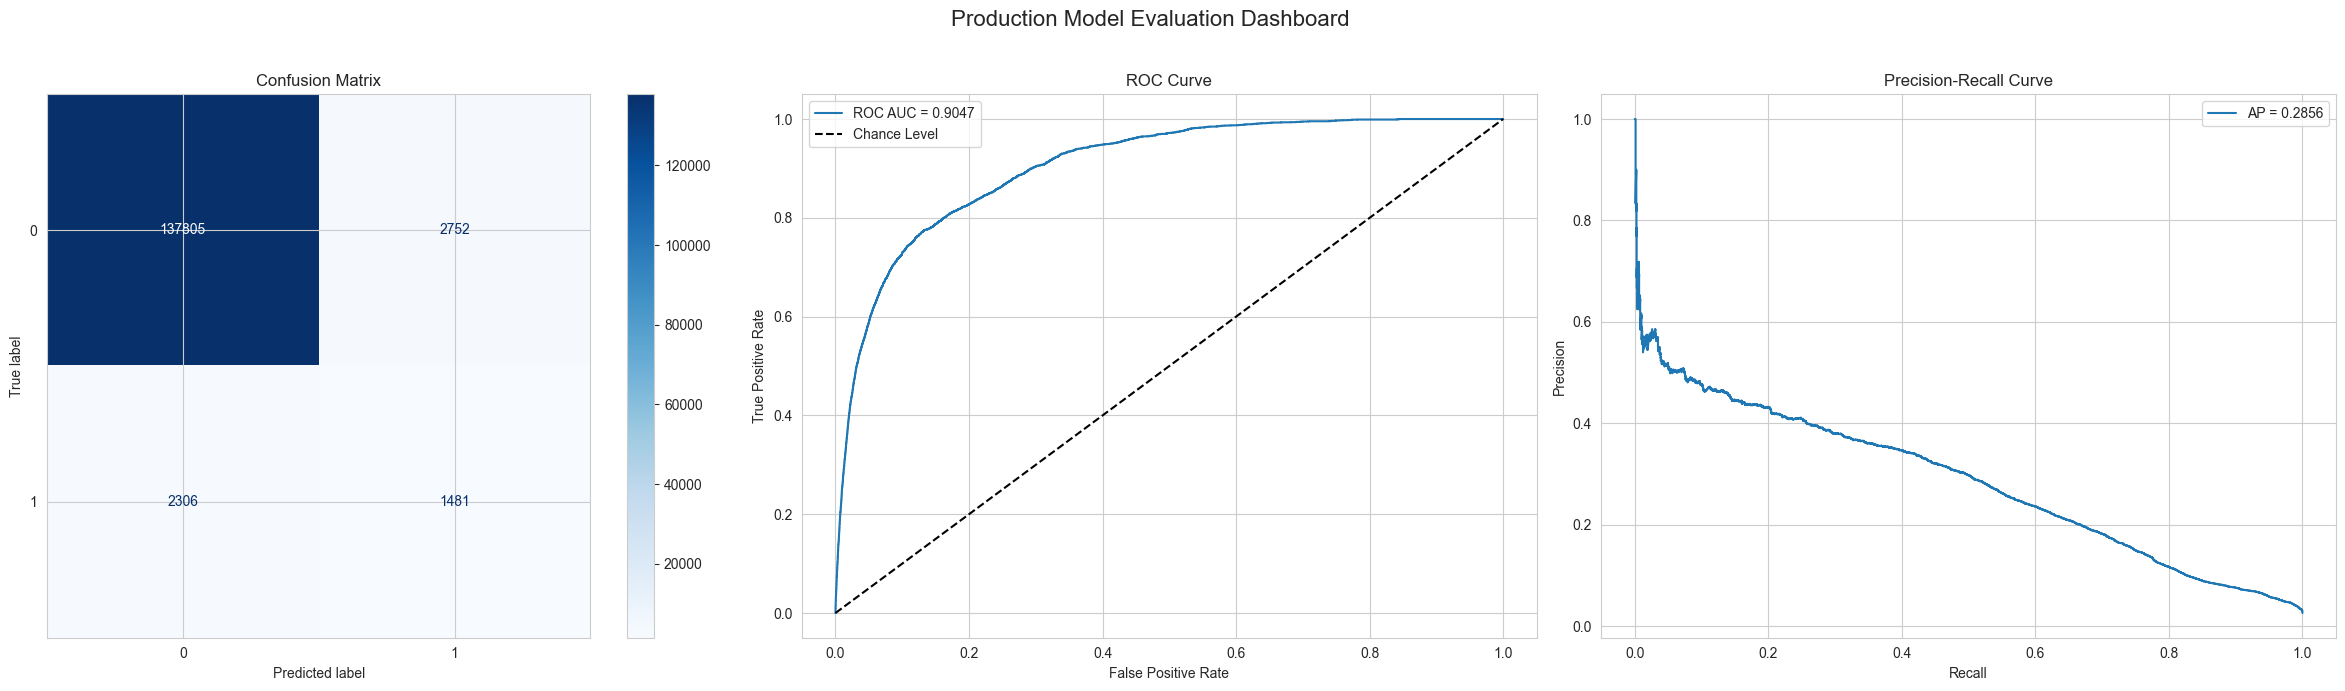
\includegraphics[width=0.85\textwidth]{LogisticRegression_evaluation_dashboard.png}
\caption{Evaluation Dashboard for Logistic Regression Model (from repository artifact).}
\end{figure}

\begin{figure}[H]
\centering
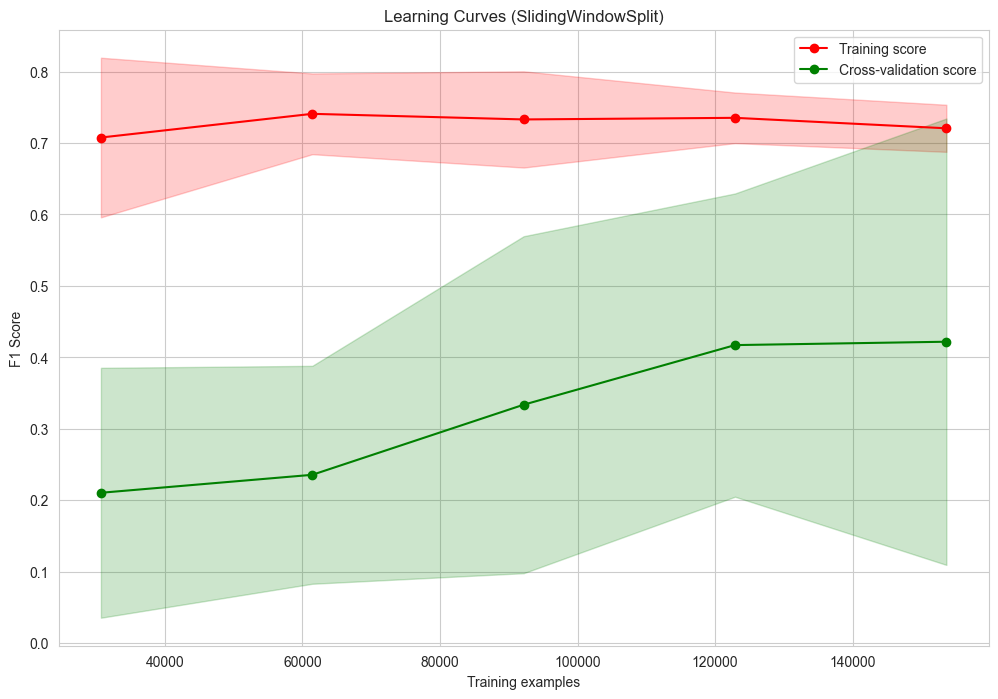
\includegraphics[width=0.7\textwidth]{LogisticRegression_learning_curve.png}
\caption{Learning curve indicating generalization behavior.}
\end{figure}

\subsection{Confusion Matrix and Curves}
Confusion matrix (threshold = 0.64), ROC curve, and Precision--Recall curve: \texttt{<INFO TO ADD>}.

\section{Explainability}

\subsection{Importance of Explainability}
Explainability is crucial in safety-related applications to build trust and allow users to understand why a particular risk assessment was made. It helps users make informed decisions and provides transparency in the model's decision-making process.

\subsection{SHAP Values}

\subsubsection{How SHAP Interprets Features}
SHAP (SHapley Additive exPlanations) values explain the contribution of each feature to a specific prediction. Positive SHAP values increase the predicted risk, while negative values decrease it.

\subsubsection{Visual Examples}

\begin{figure}[H]
\centering
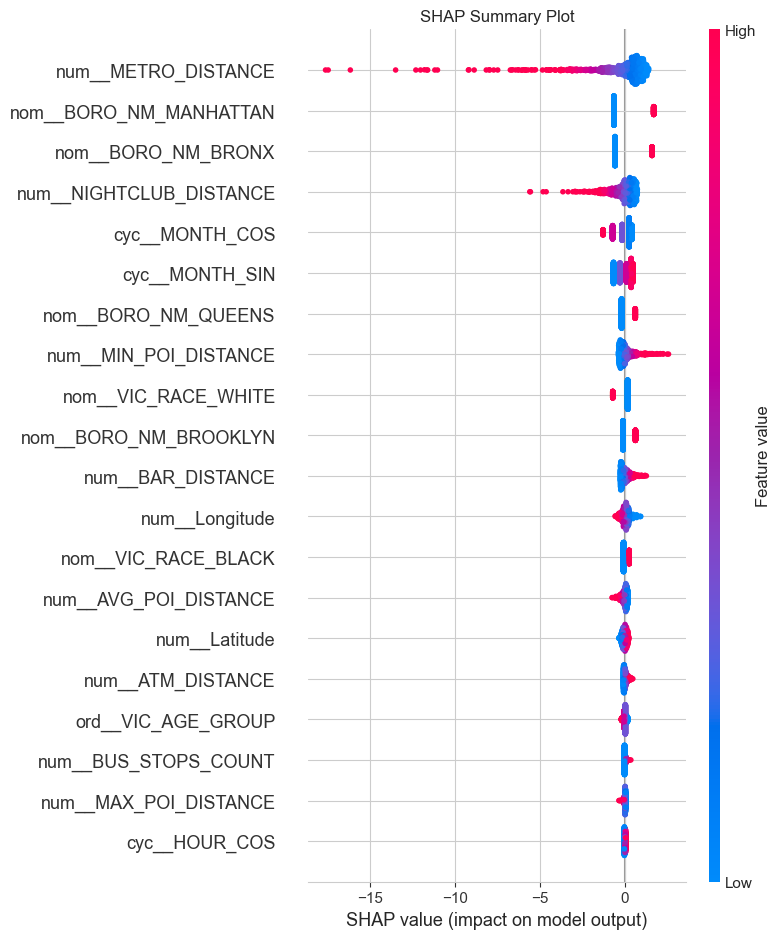
\includegraphics[width=0.8\textwidth]{LogisticRegression_shap_summary.png}
\caption{SHAP Summary Plot Showing Feature Importance}
\end{figure}

\begin{figure}[H]
\centering
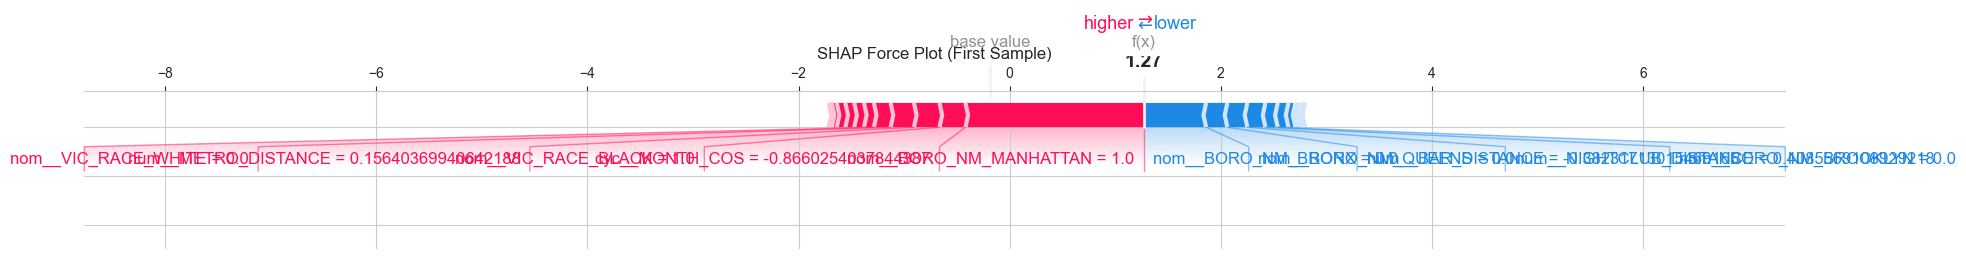
\includegraphics[width=0.8\textwidth]{LogisticRegression_shap_force.png}
\caption{SHAP Force Plot for Individual Prediction}
\end{figure}

\subsubsection{Practical Example}
Concrete SHAP contribution values for a specific scenario: \texttt{<INFO TO ADD>}.

\begin{figure}[H]
\centering
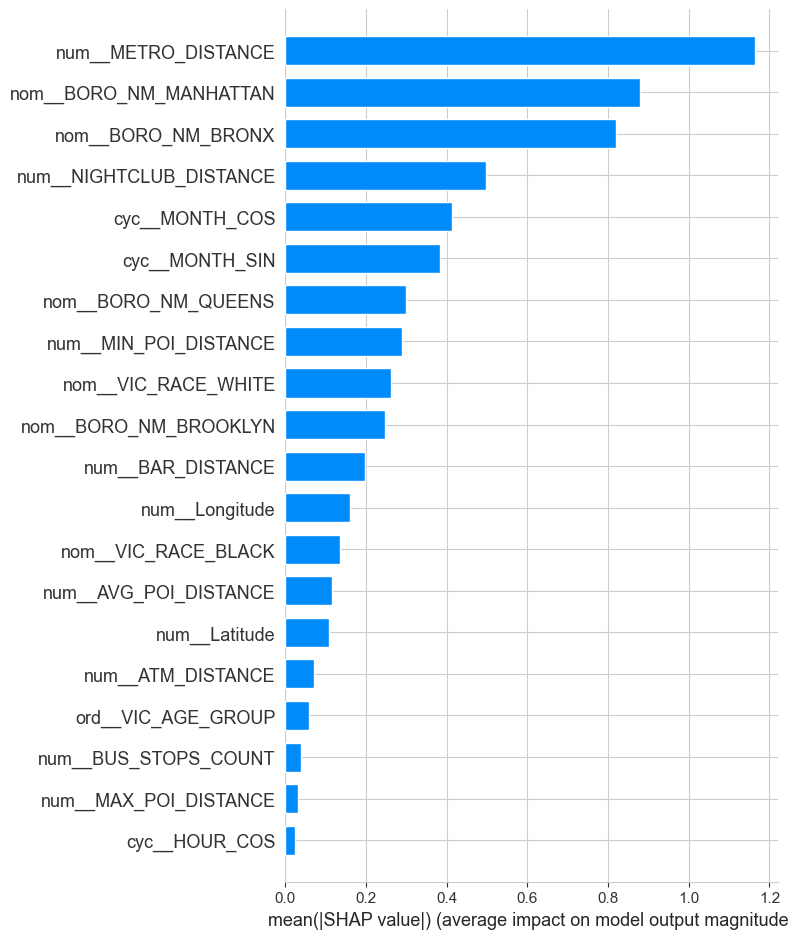
\includegraphics[width=0.8\textwidth]{LogisticRegression_shap_feature_importance.png}
\caption{SHAP Feature Importance Plot}
\end{figure}

\begin{figure}[H]
\centering
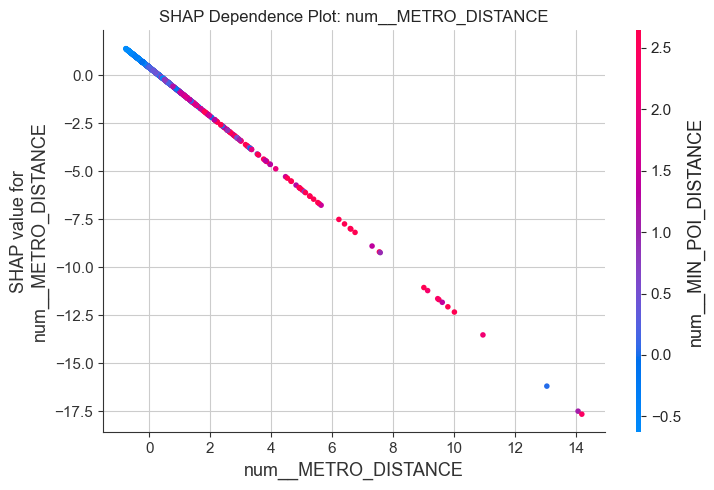
\includegraphics[width=0.75\textwidth]{LogisticRegression_shap_dependence.png}
\caption{SHAP dependence plot for a key feature.}
\end{figure}

\subsection{Threshold Optimization Policy}
\label{sec:threshold}
The decision threshold was tuned to maximize F1 on validation outputs. The selected threshold is \textbf{0.64}. The threshold optimization artifact is included below.

\begin{figure}[H]
\centering
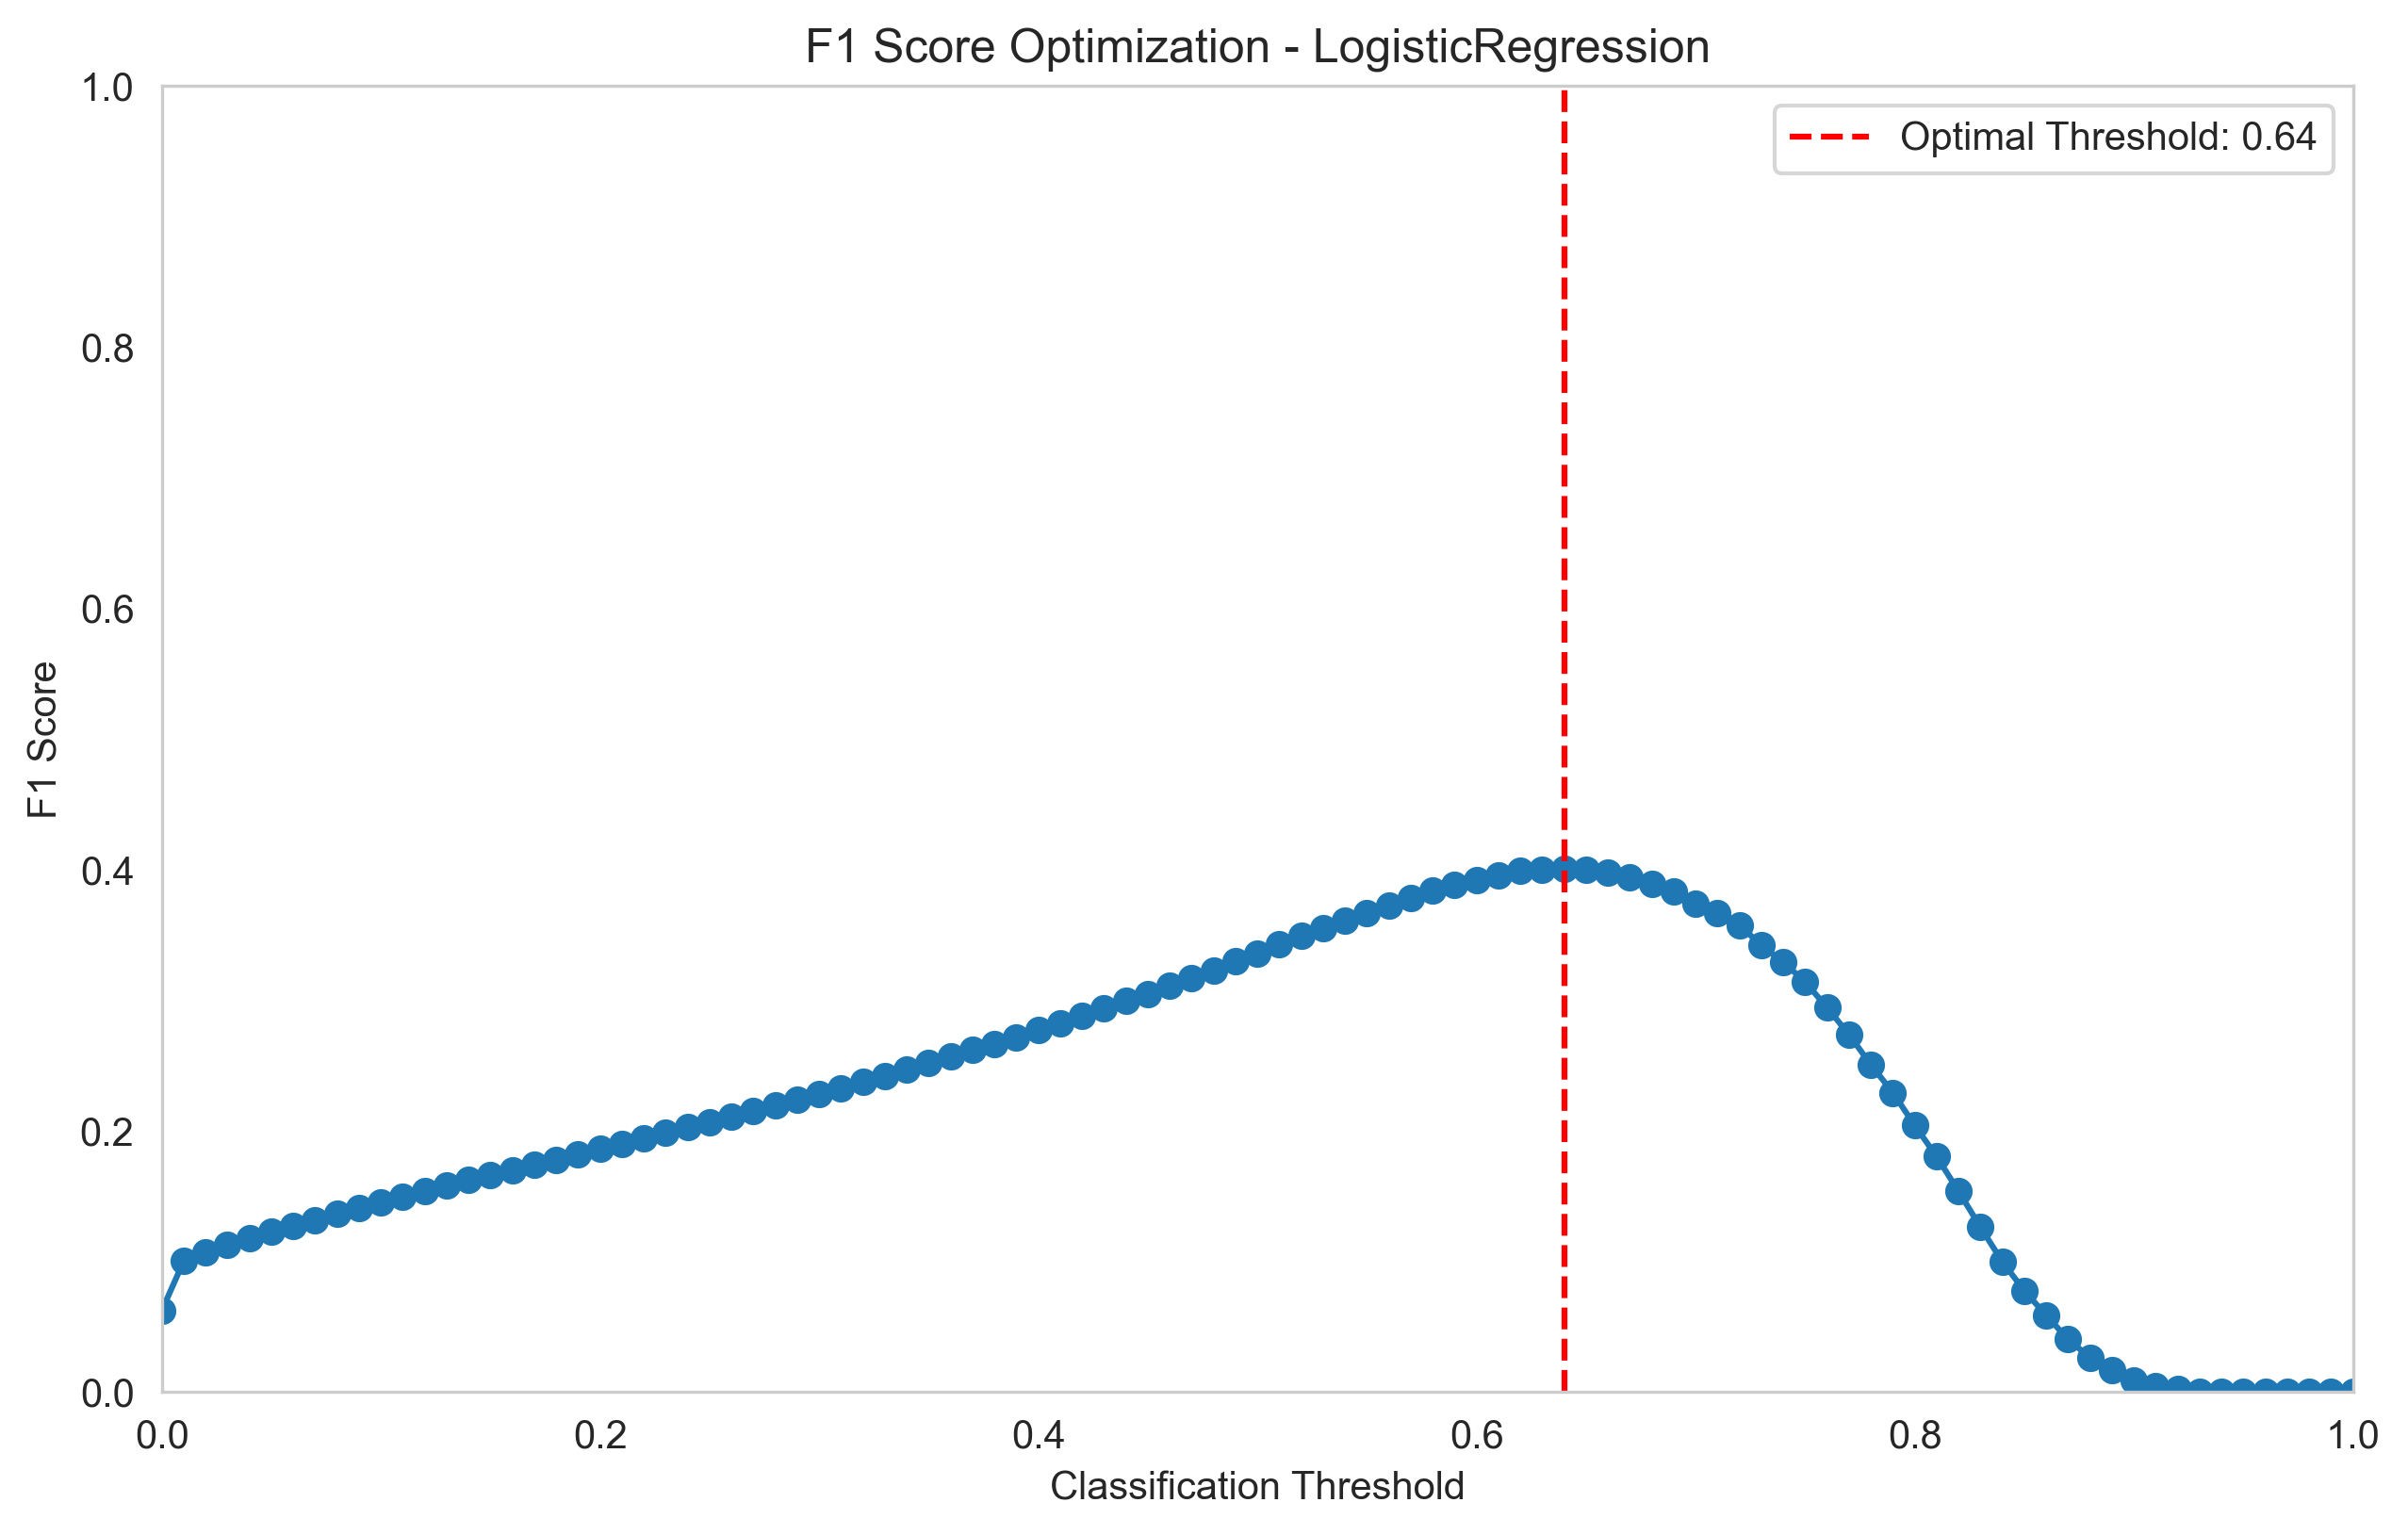
\includegraphics[width=0.8\textwidth]{LogisticRegression_f1_threshold_optimization.png}
\caption{Threshold optimization curve (F1 vs. threshold).}
\end{figure}

\section{Frequent Pattern Analysis}

\subsection{Technique Description}
The system employs Frequent Itemset Mining using the FP-Growth algorithm (\texttt{mlxtend.frequent\_patterns}) to discover association rules and patterns in crime data.\footnote{See \texttt{Notebooks/PatternAnalysis/PatternAnalysis.ipynb}.} This technique identifies combinations of factors that frequently occur together, providing insights beyond individual predictions.

\subsection{Application to Crime Context}
Pattern analysis helps identify recurring crime patterns, such as:
- Specific crime types occurring in certain locations at particular times.
- Combinations of victim demographics and crime circumstances.
- Temporal and spatial correlations in criminal activity.

\subsection{Intuitive Examples}
\begin{itemize}
\item \textbf{Pattern 1}: In Manhattan, during weekend evenings (8 PM - 12 AM), thefts from vehicles are 3 times more likely near bars and nightclubs.
\item \textbf{Pattern 2}: Near subway stations after 10 PM, robberies involving young male victims increase by 40\%.
\item \textbf{Pattern 3}: In summer months, assaults in outdoor locations spike during late-night hours.
\end{itemize}

These patterns provide contextual information that complements the binary risk prediction, helping users understand the types of risks they might encounter.

\subsection{Mining Configuration}
From the repository notebook defaults:
\begin{itemize}
	\item Global minimum support: \texttt{0.5}
	\item Slice minimum support range: \texttt{(0.01, 0.02)}
	\item Minimum confidence: \texttt{0.40}
	\item Maximum itemset length: \texttt{4}
\end{itemize}

Top-N rules tables and visual summaries: \texttt{<INFO TO ADD>}.

\subsection{Value for Tourists}
While the ML model provides a risk score, pattern analysis offers:
\begin{itemize}
\item Specific crime type warnings.
\item Temporal trends for planning activities.
\item Location-based insights for route planning.
\end{itemize}

\section{User Interface}

\subsection{Input Methods}
\begin{itemize}
\item \textbf{Automatic GPS}: The system can automatically detect the user's location via GPS.
\item \textbf{Manual Input}: Users can manually enter coordinates or select locations on a map.
\end{itemize}

\subsection{Output Methods}
\begin{itemize}
\item \textbf{Textual Output}: Simple HIGH RISK / LOW RISK display.
\item \textbf{Probabilistic Output}: Confidence scores for the prediction.
\end{itemize}

\subsection{Future Extensions}
Potential UI improvements include:
\begin{itemize}
\item Interactive maps with color-coded risk zones.
\item Real-time alerts based on user movement.
\item Historical trend visualizations.
\end{itemize}

\section{System Limitations}

\subsection{Data Biases}
\begin{itemize}
\item Historical data may have biases due to varying reporting rates across neighborhoods.
\item Some areas might be under-monitored, leading to incomplete data.
\end{itemize}

\subsection{False Positives/Negatives}
\begin{itemize}
\item The model may occasionally misclassify safe areas as high risk or vice versa.
\item Current precision (\textasciitilde35\%) indicates room for improvement in reducing false alarms.
\item Positive class prevalence during evaluation: \texttt{<INFO TO ADD>} (helps contextualize accuracy vs. recall).
\end{itemize}

\subsection{Data Coverage Gaps}
\begin{itemize}
\item Limited coverage in certain geographic areas.
\item Potential gaps in real-time data integration.
\end{itemize}



\section{Future Extensions}

\subsection{Interactive Maps}
Integration with mapping services to visualize risk zones in real-time.

\subsection{Probabilistic Output}
Replace binary classification with probability scores for more nuanced risk assessment.

\subsection{Real-time Data Integration}
Incorporate live data feeds from police reports, social media, and IoT sensors.

\subsection{Enhanced Pattern Mining}
Develop more sophisticated pattern analysis with:
\begin{itemize}
\item Sequential pattern mining for crime progression.
\item Multi-feature correlations.
\item Predictive pattern-based alerts.
\end{itemize}

\section{Conclusion}

\subsection{Benefits Summary}
The Crime Risk Prediction System provides tourists with data-driven insights to enhance their safety in New York City. By combining machine learning predictions with explainability and pattern analysis, it offers both immediate risk assessments and deeper contextual understanding.

\subsection{Potential Applications}
Beyond tourism, this system has applications for:
\begin{itemize}
\item Urban planning and safety improvements.
\item Law enforcement resource allocation.
\item Insurance risk assessment.
\item Real estate safety evaluations.
\end{itemize}

\subsection{Long-term Vision}
\section{Appendix A: Preprocessing and EDA Figures}

\begin{figure}[H]
\centering
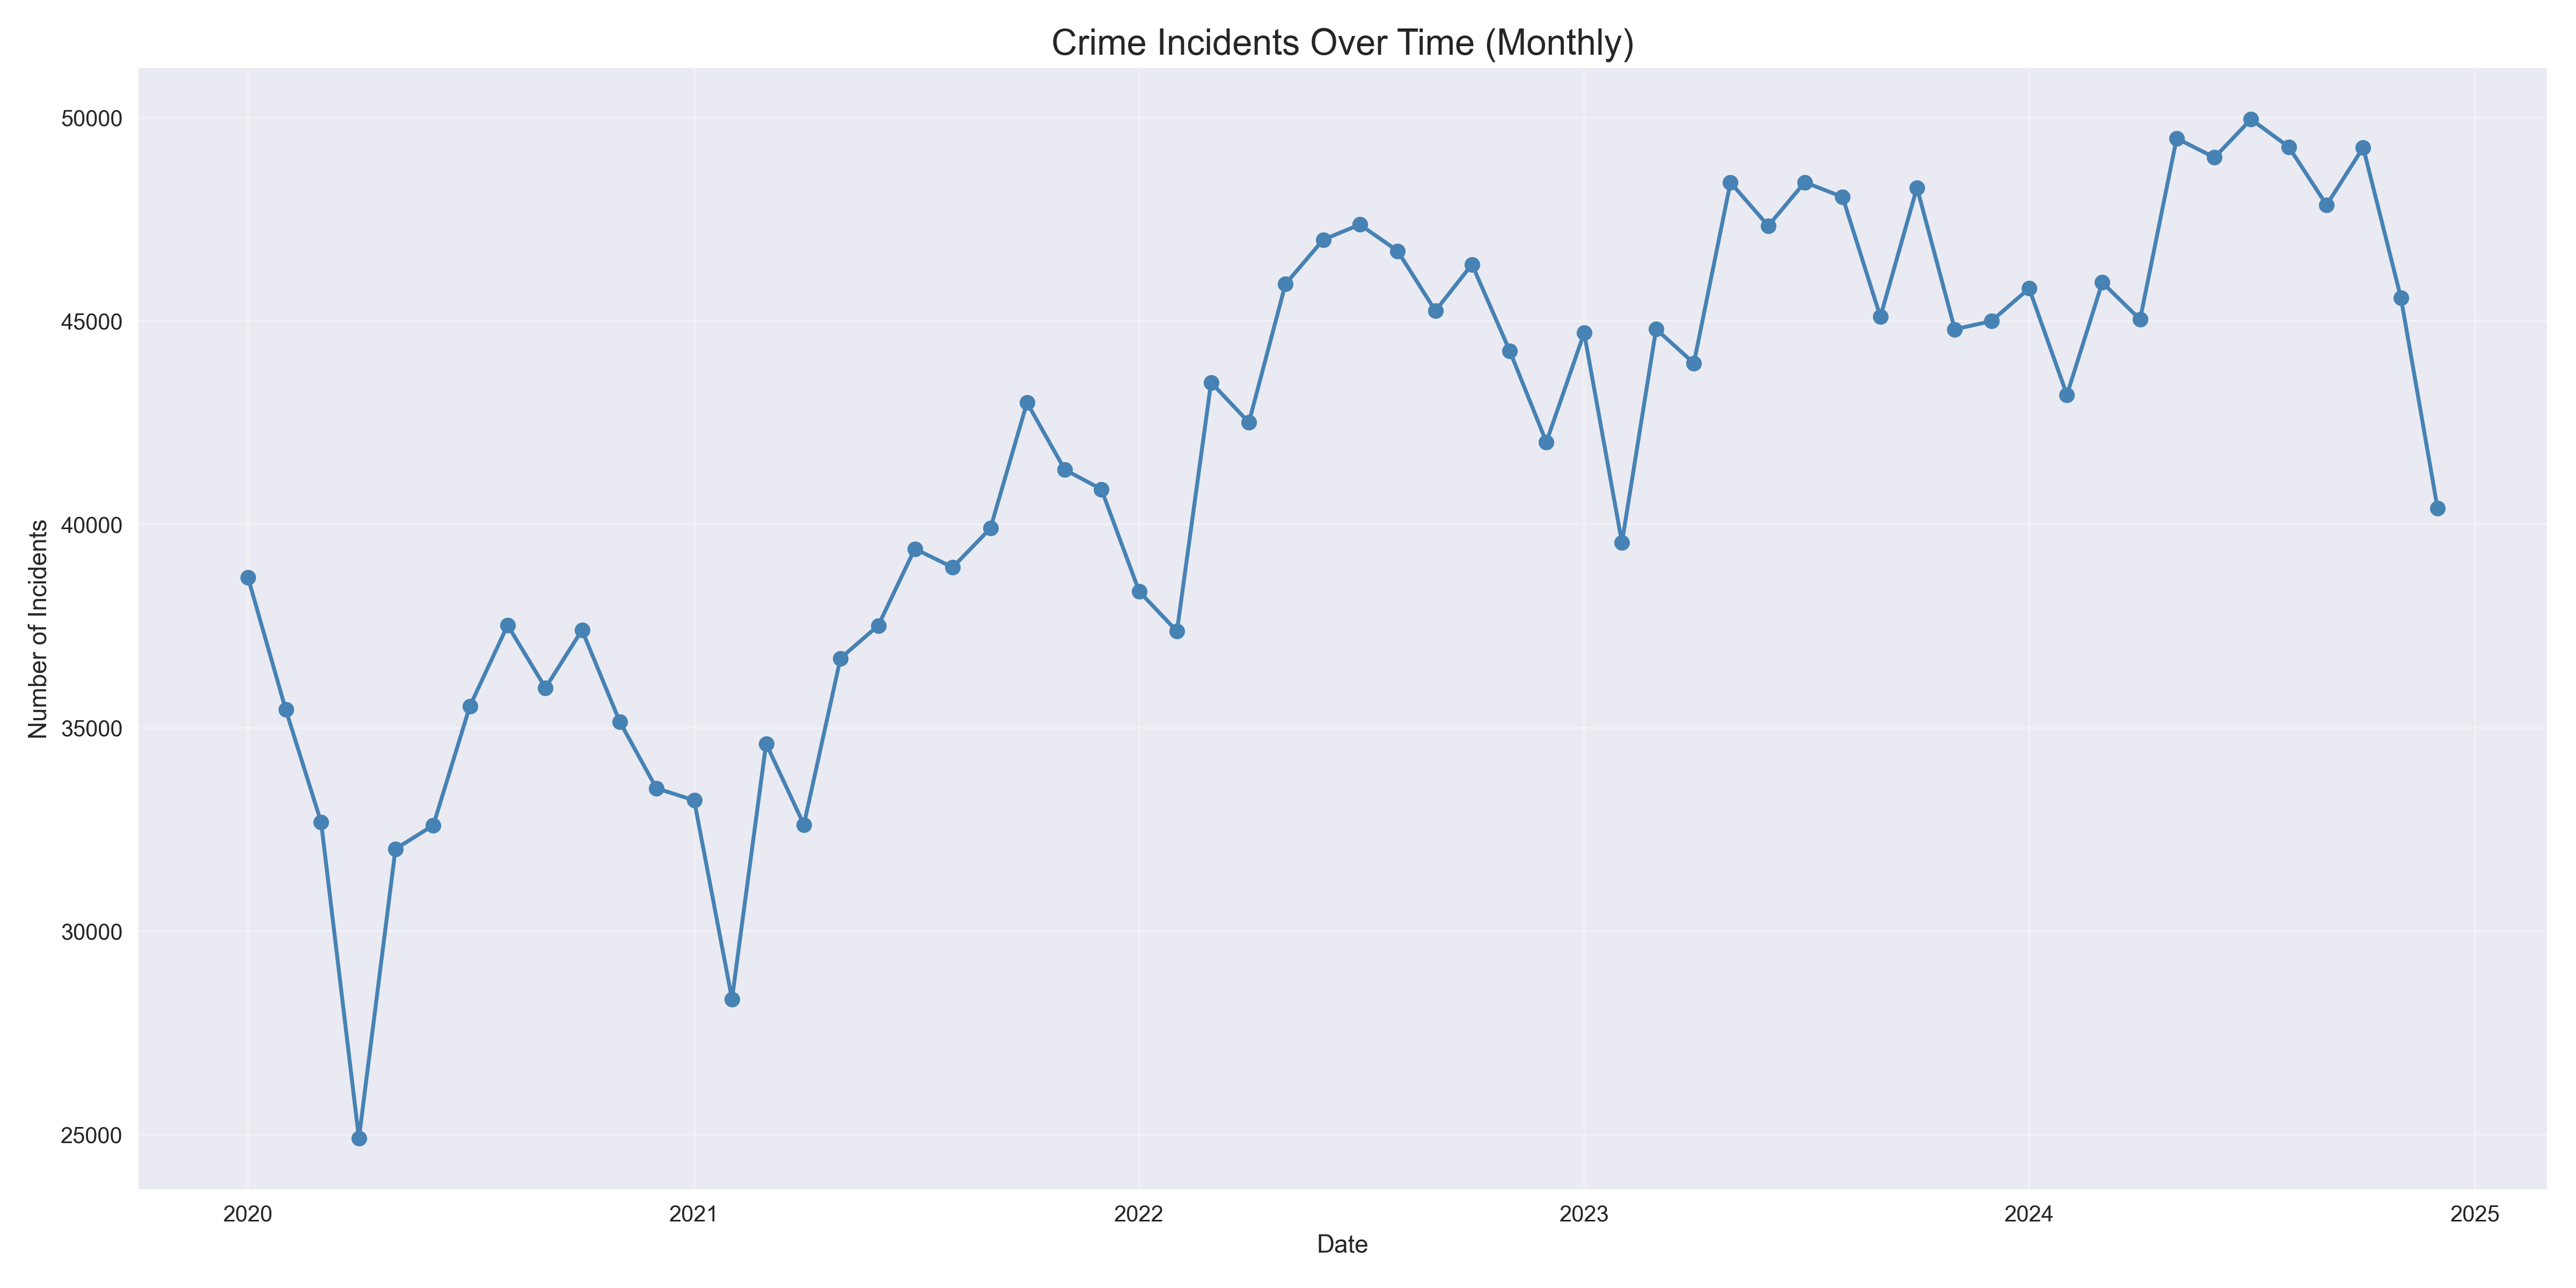
\includegraphics[width=0.75\textwidth]{crime_trends_over_time.png}
\caption{Crime trends over time (aggregated).}
\end{figure}

\begin{figure}[H]
\centering
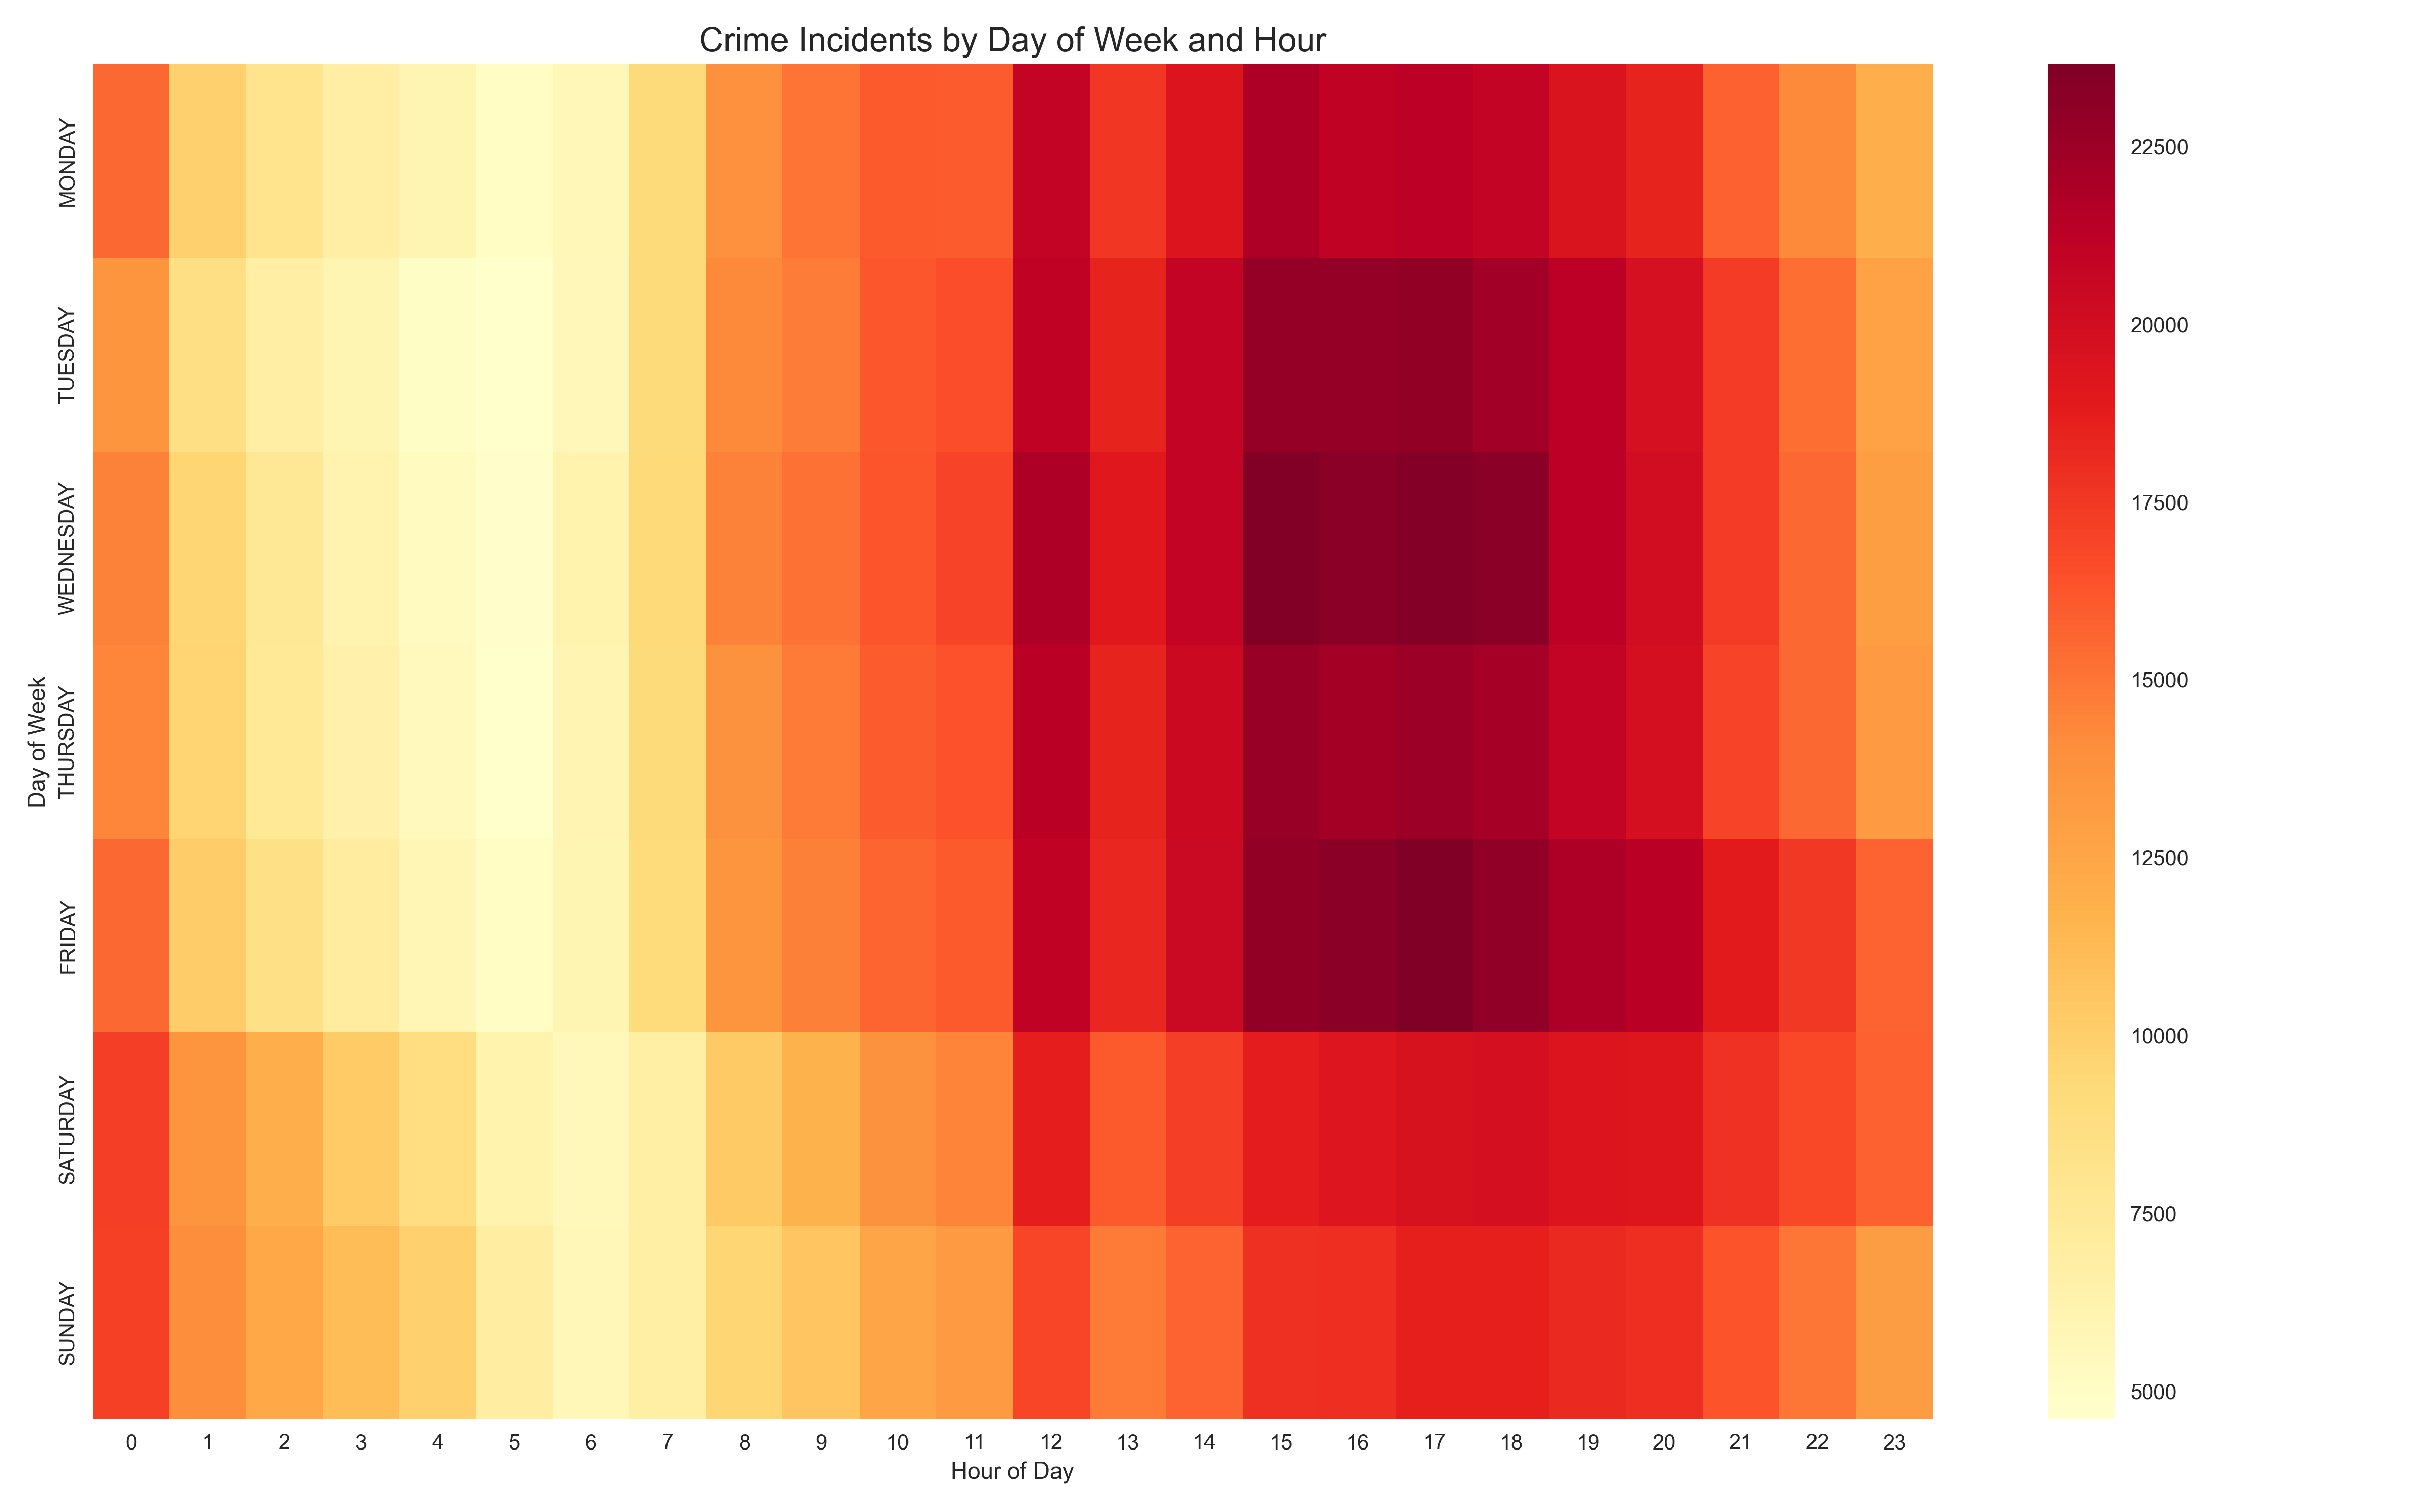
\includegraphics[width=0.75\textwidth]{crime_heatmap_day_hour.png}
\caption{Heatmap of crime counts by weekday and hour.}
\end{figure}

\begin{figure}[H]
\centering
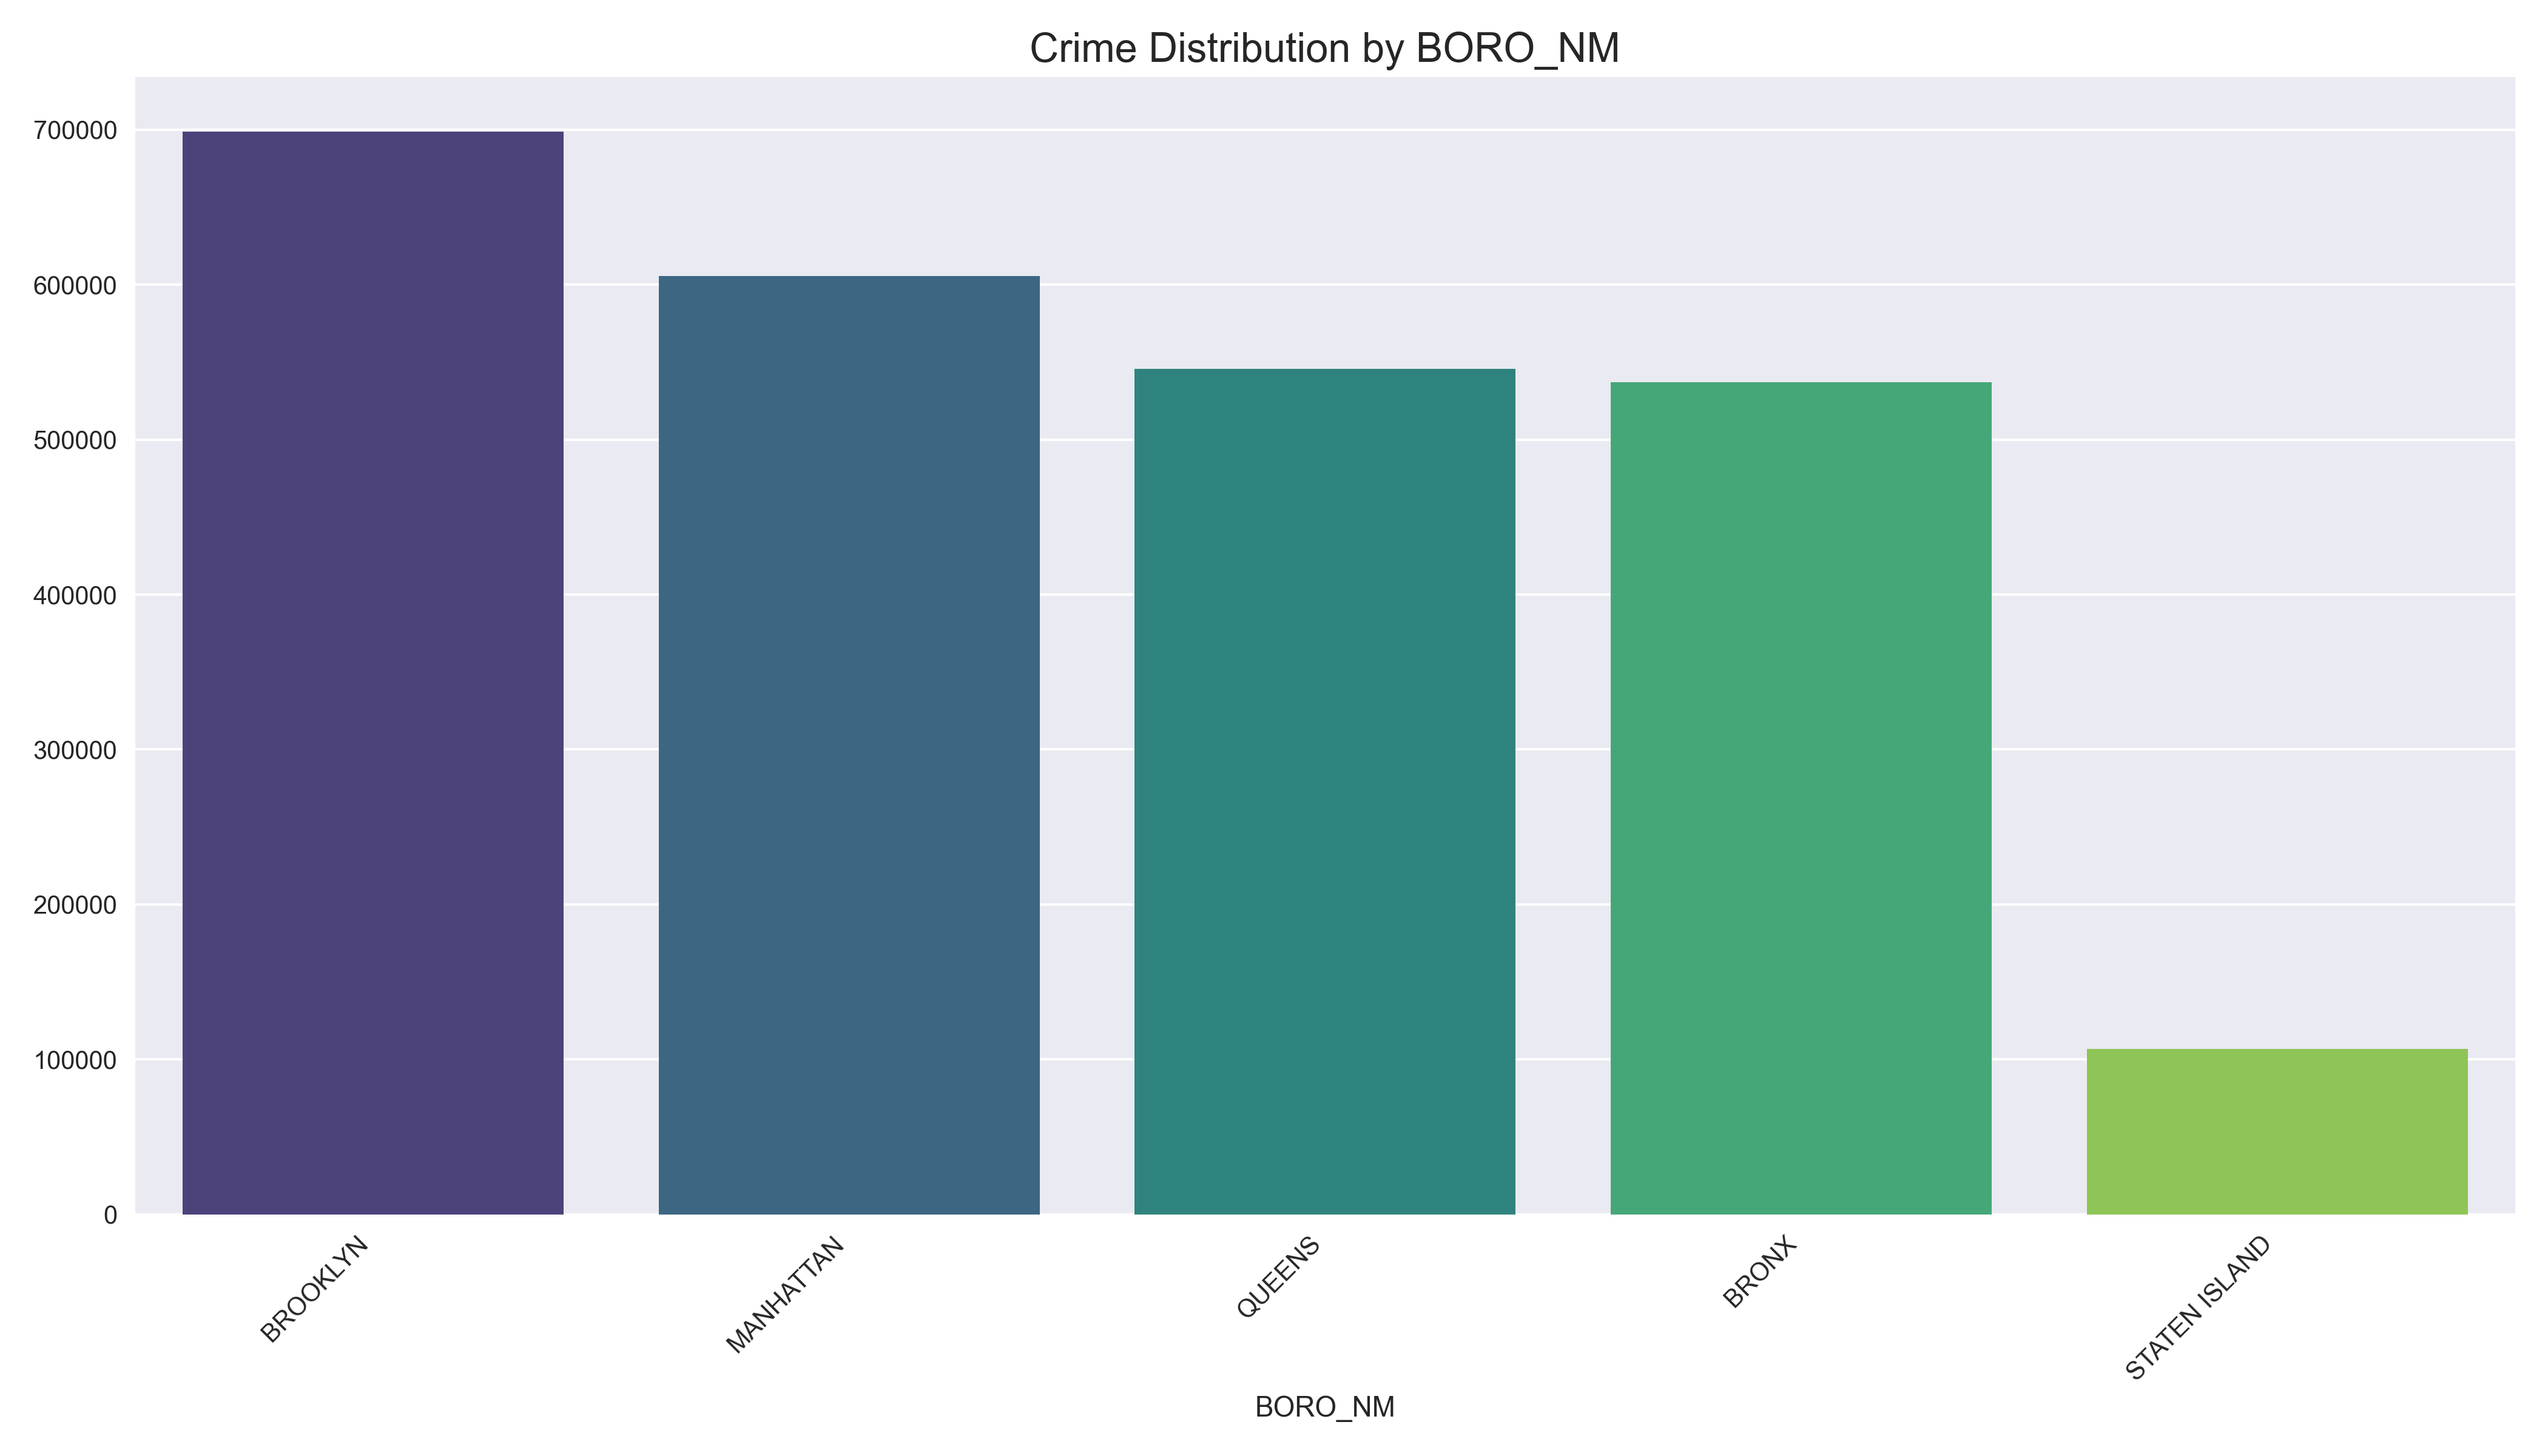
\includegraphics[width=0.45\textwidth]{crime_location_bar_chart_BORO_NM.png}
\hfill
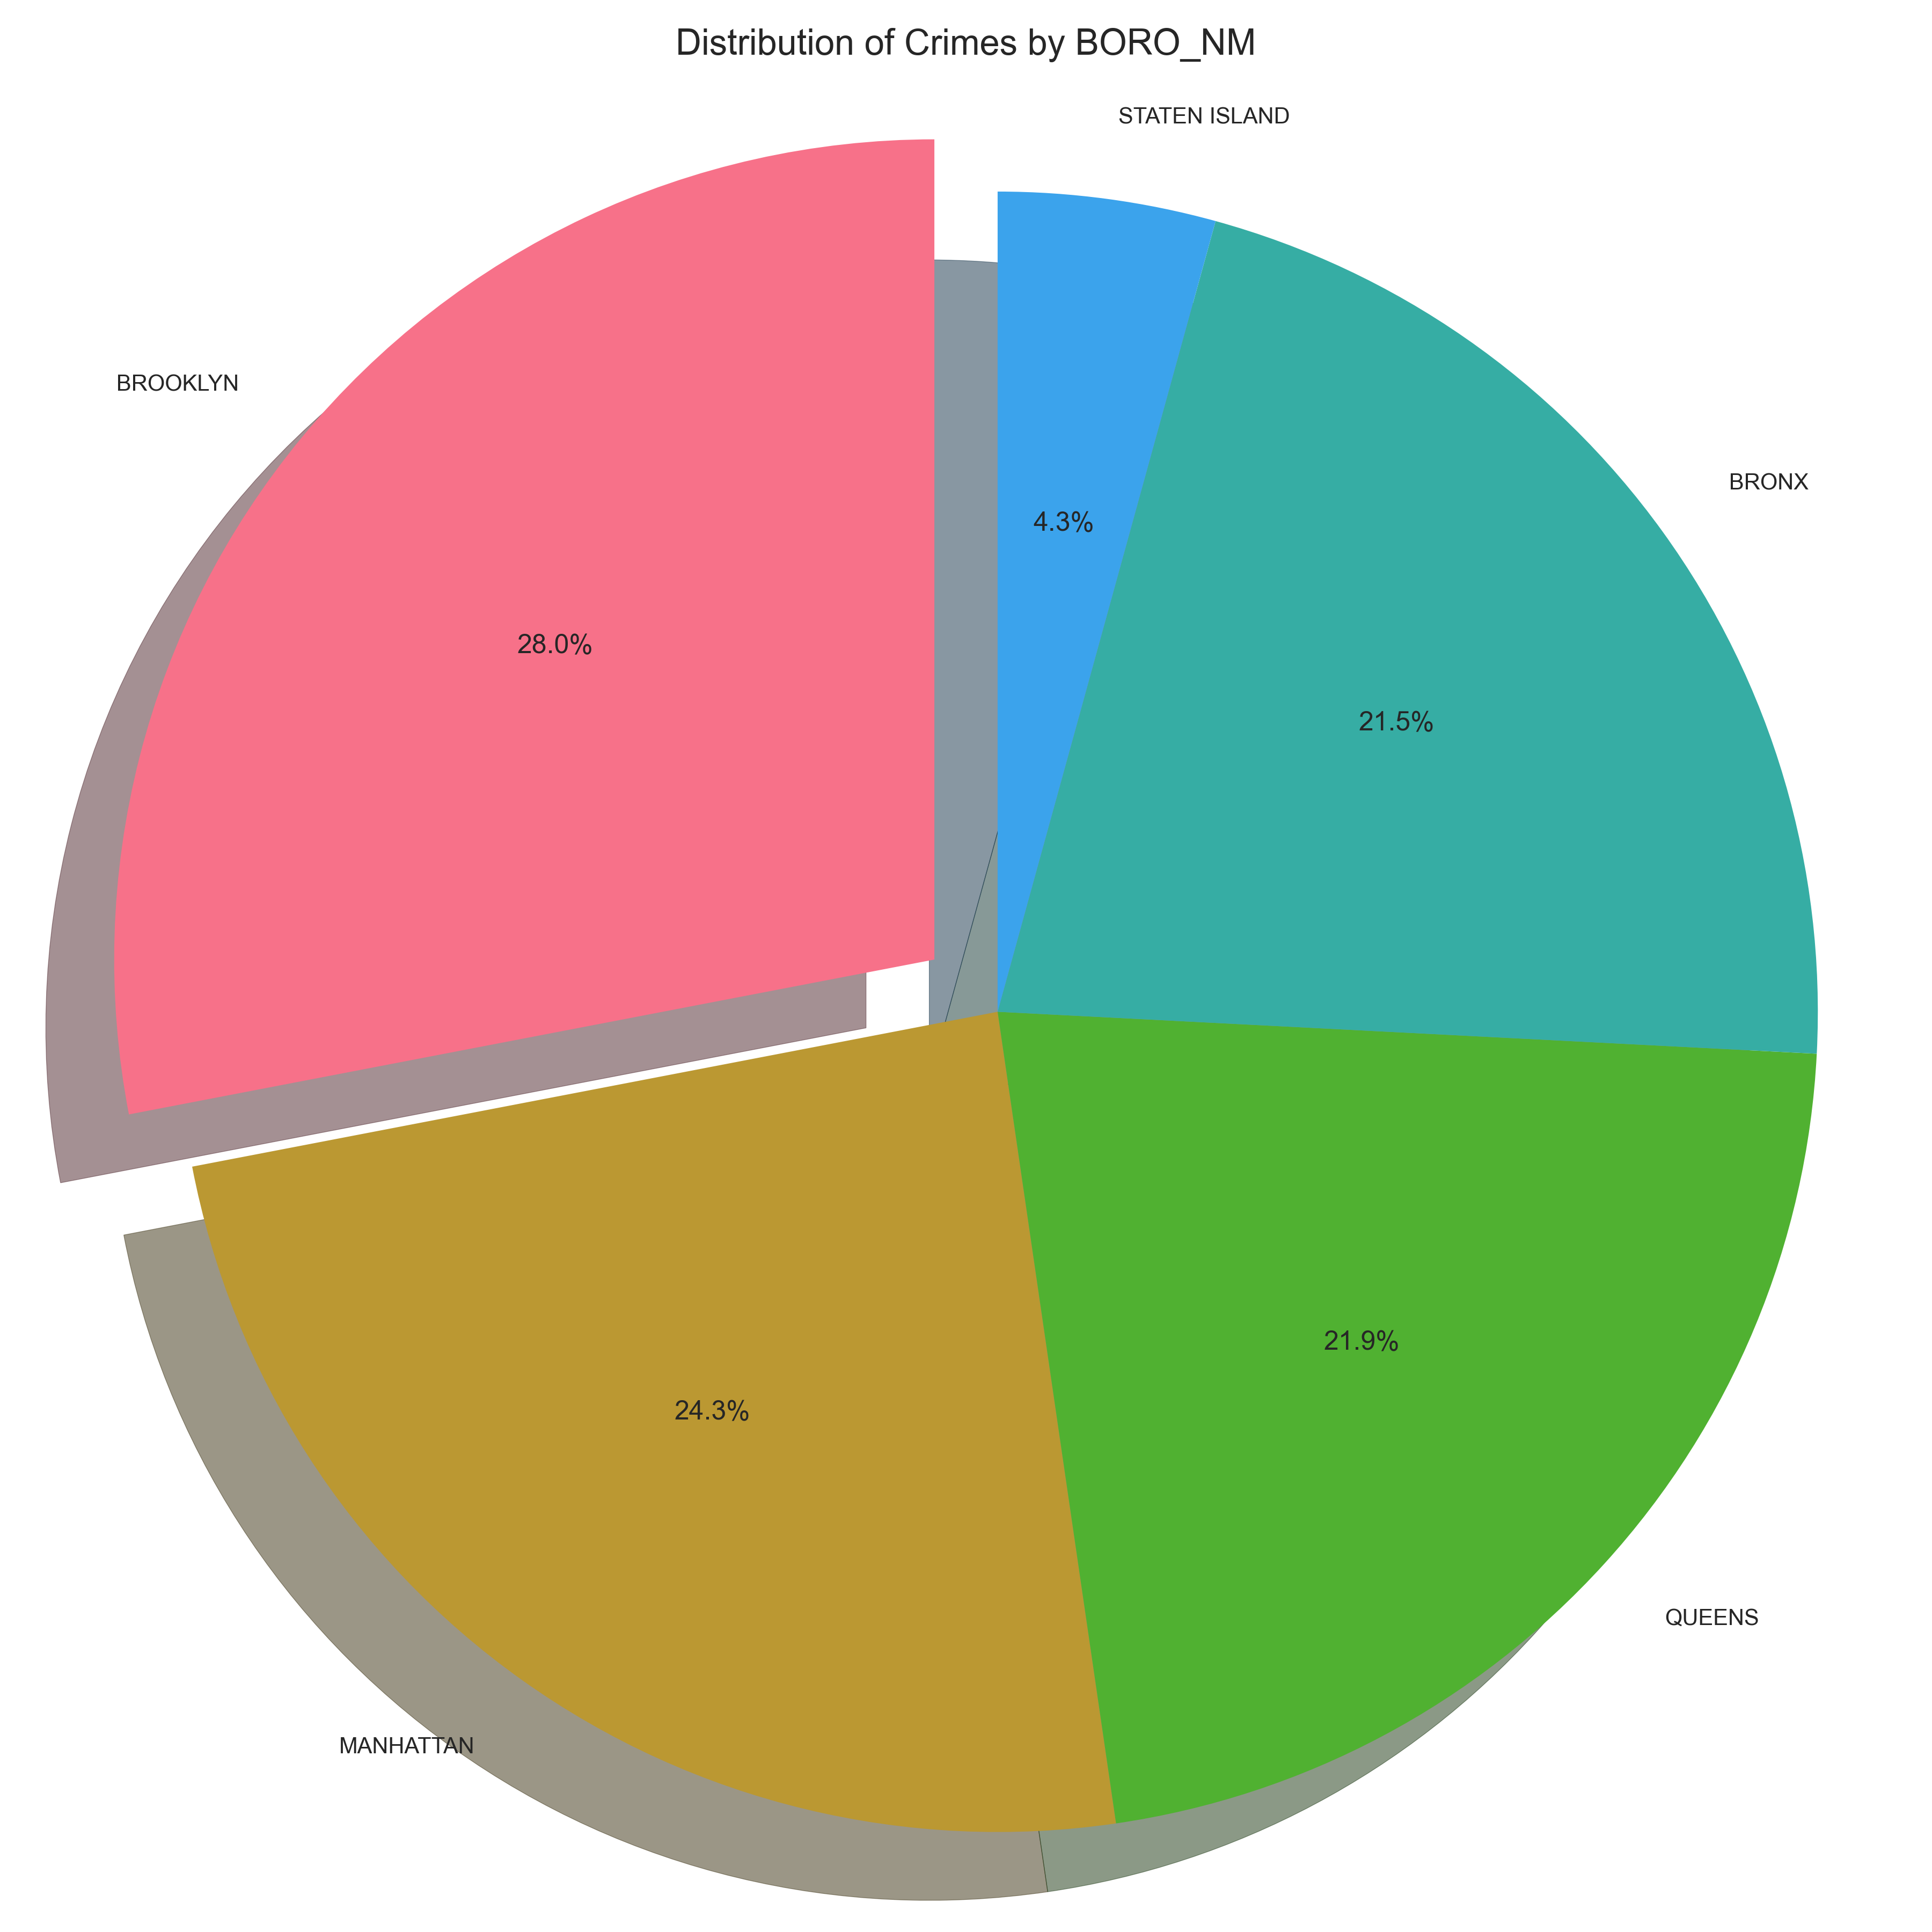
\includegraphics[width=0.45\textwidth]{crime_location_pie_chart_BORO_NM.png}
\caption{Crime distribution by borough.}
\end{figure}

\begin{figure}[H]
\centering
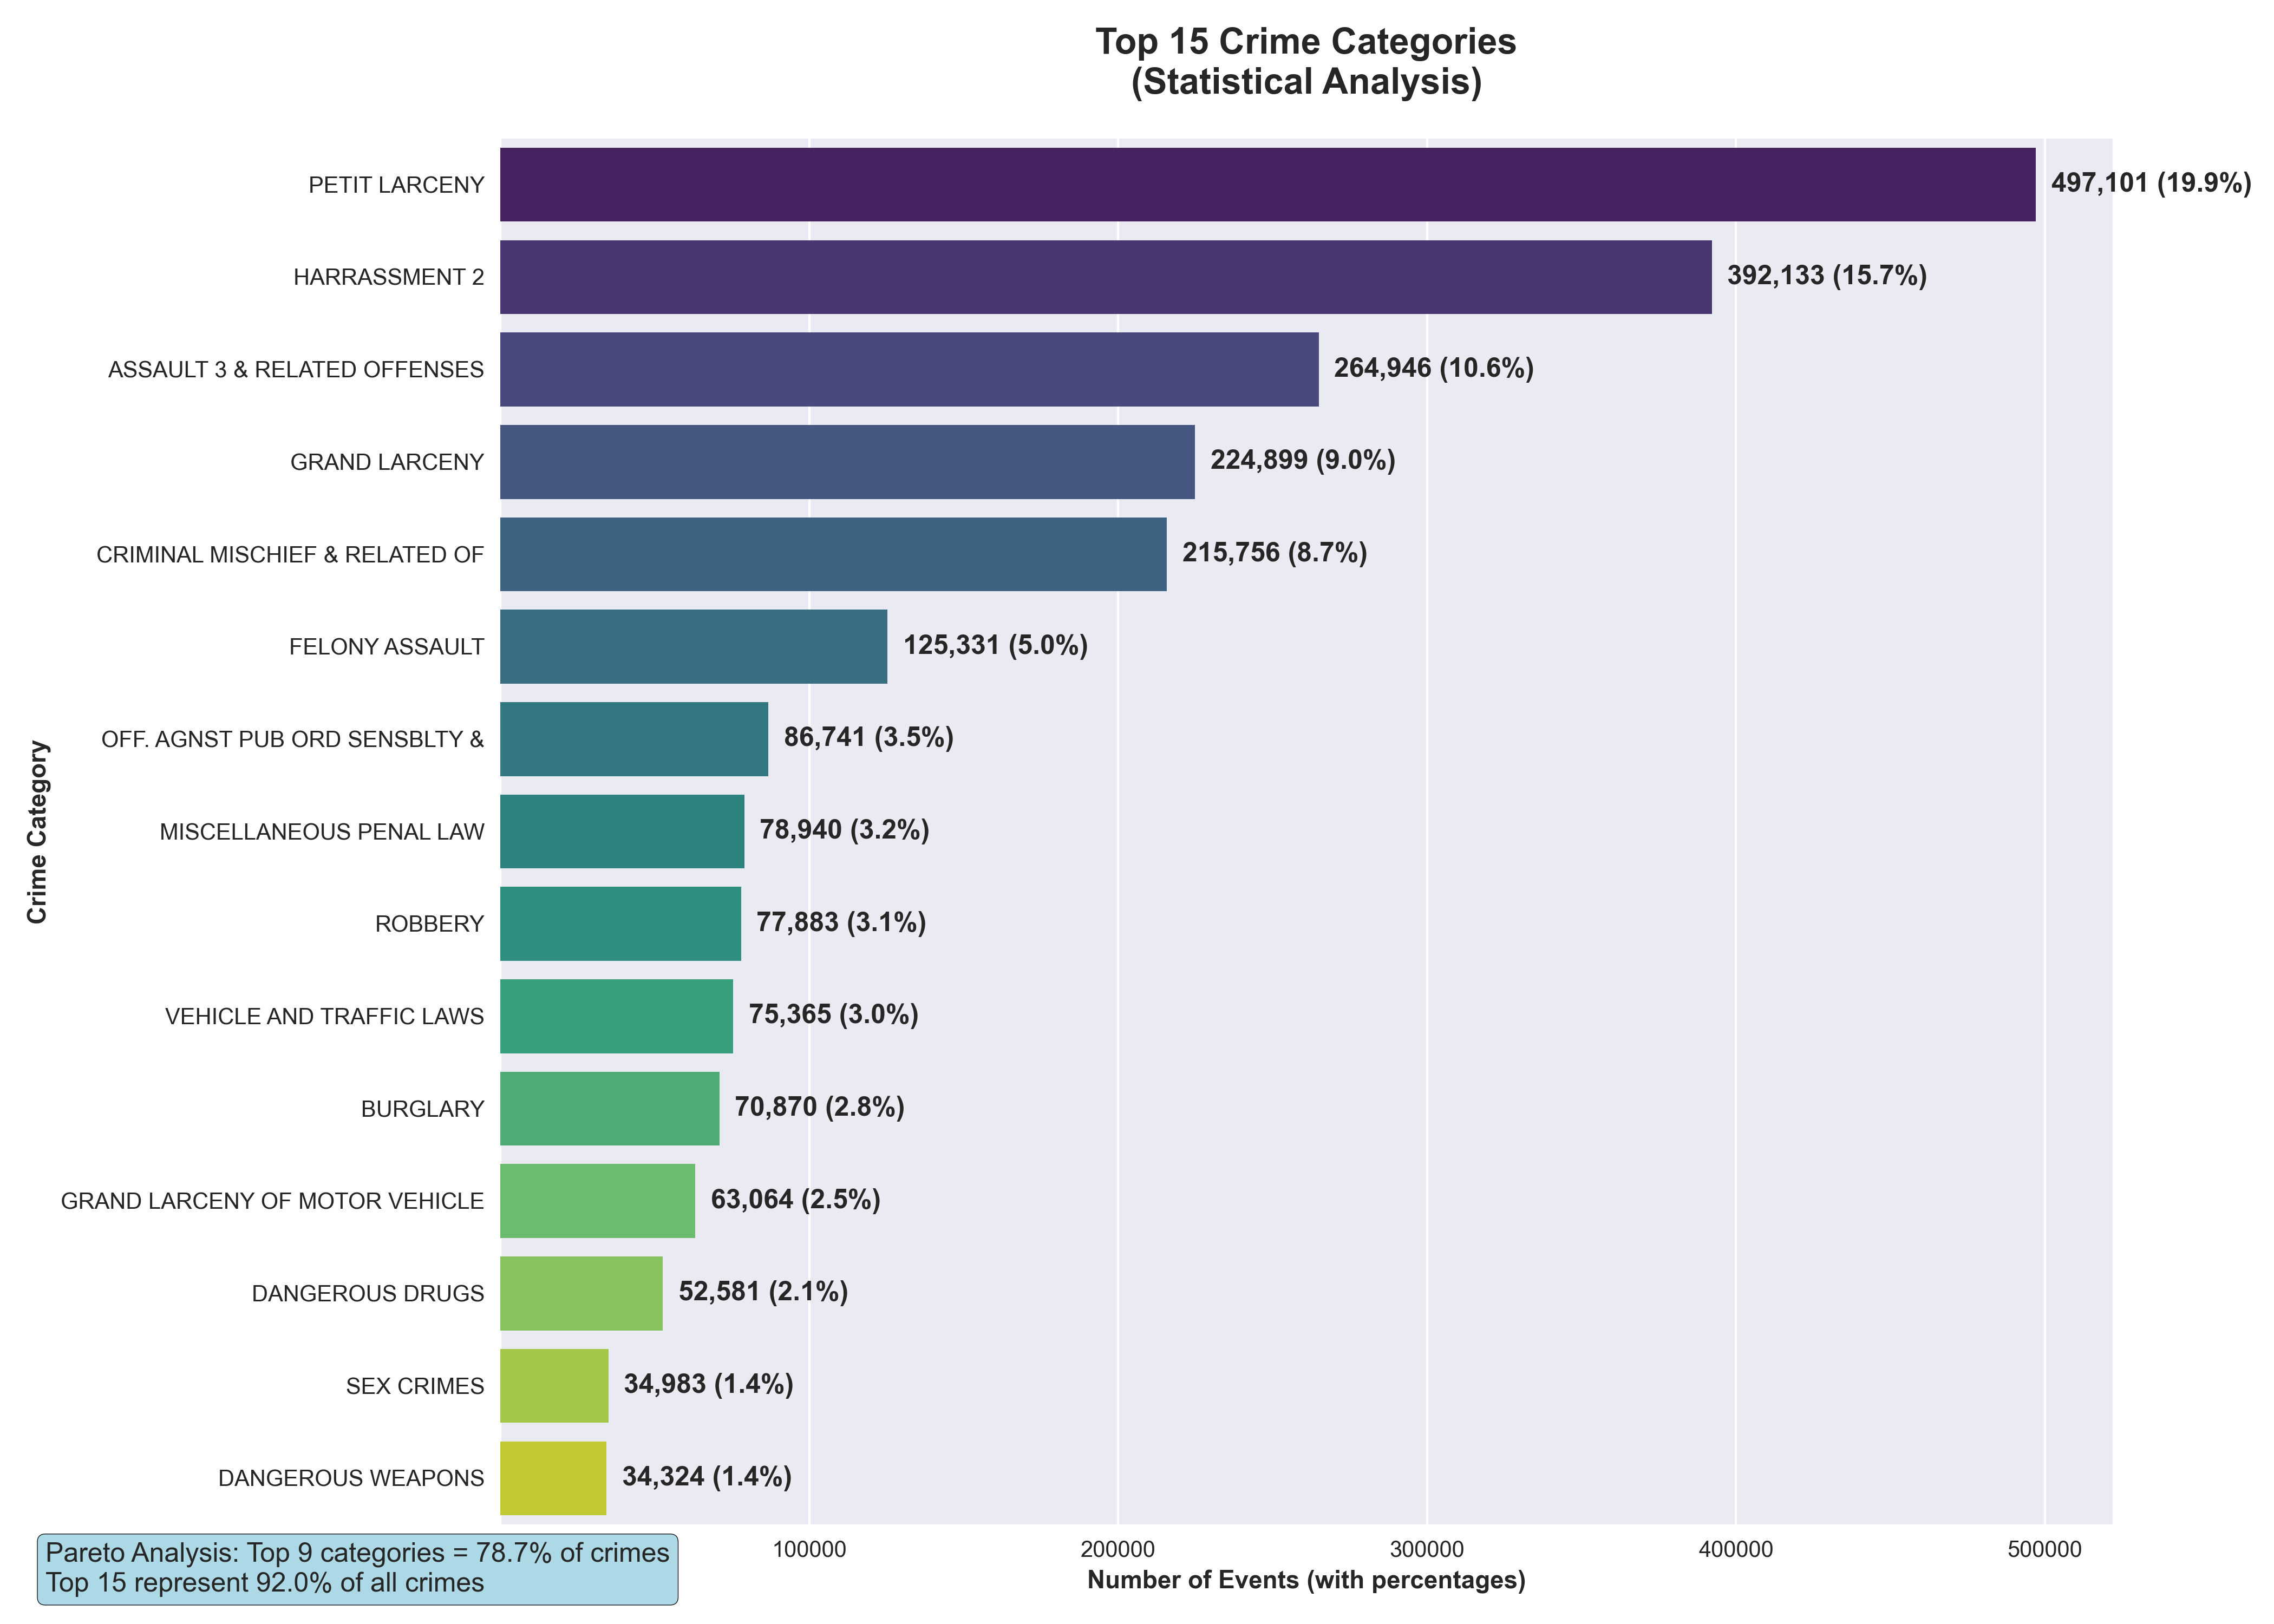
\includegraphics[width=0.45\textwidth]{crime_types_bar_chart.png}\hfill
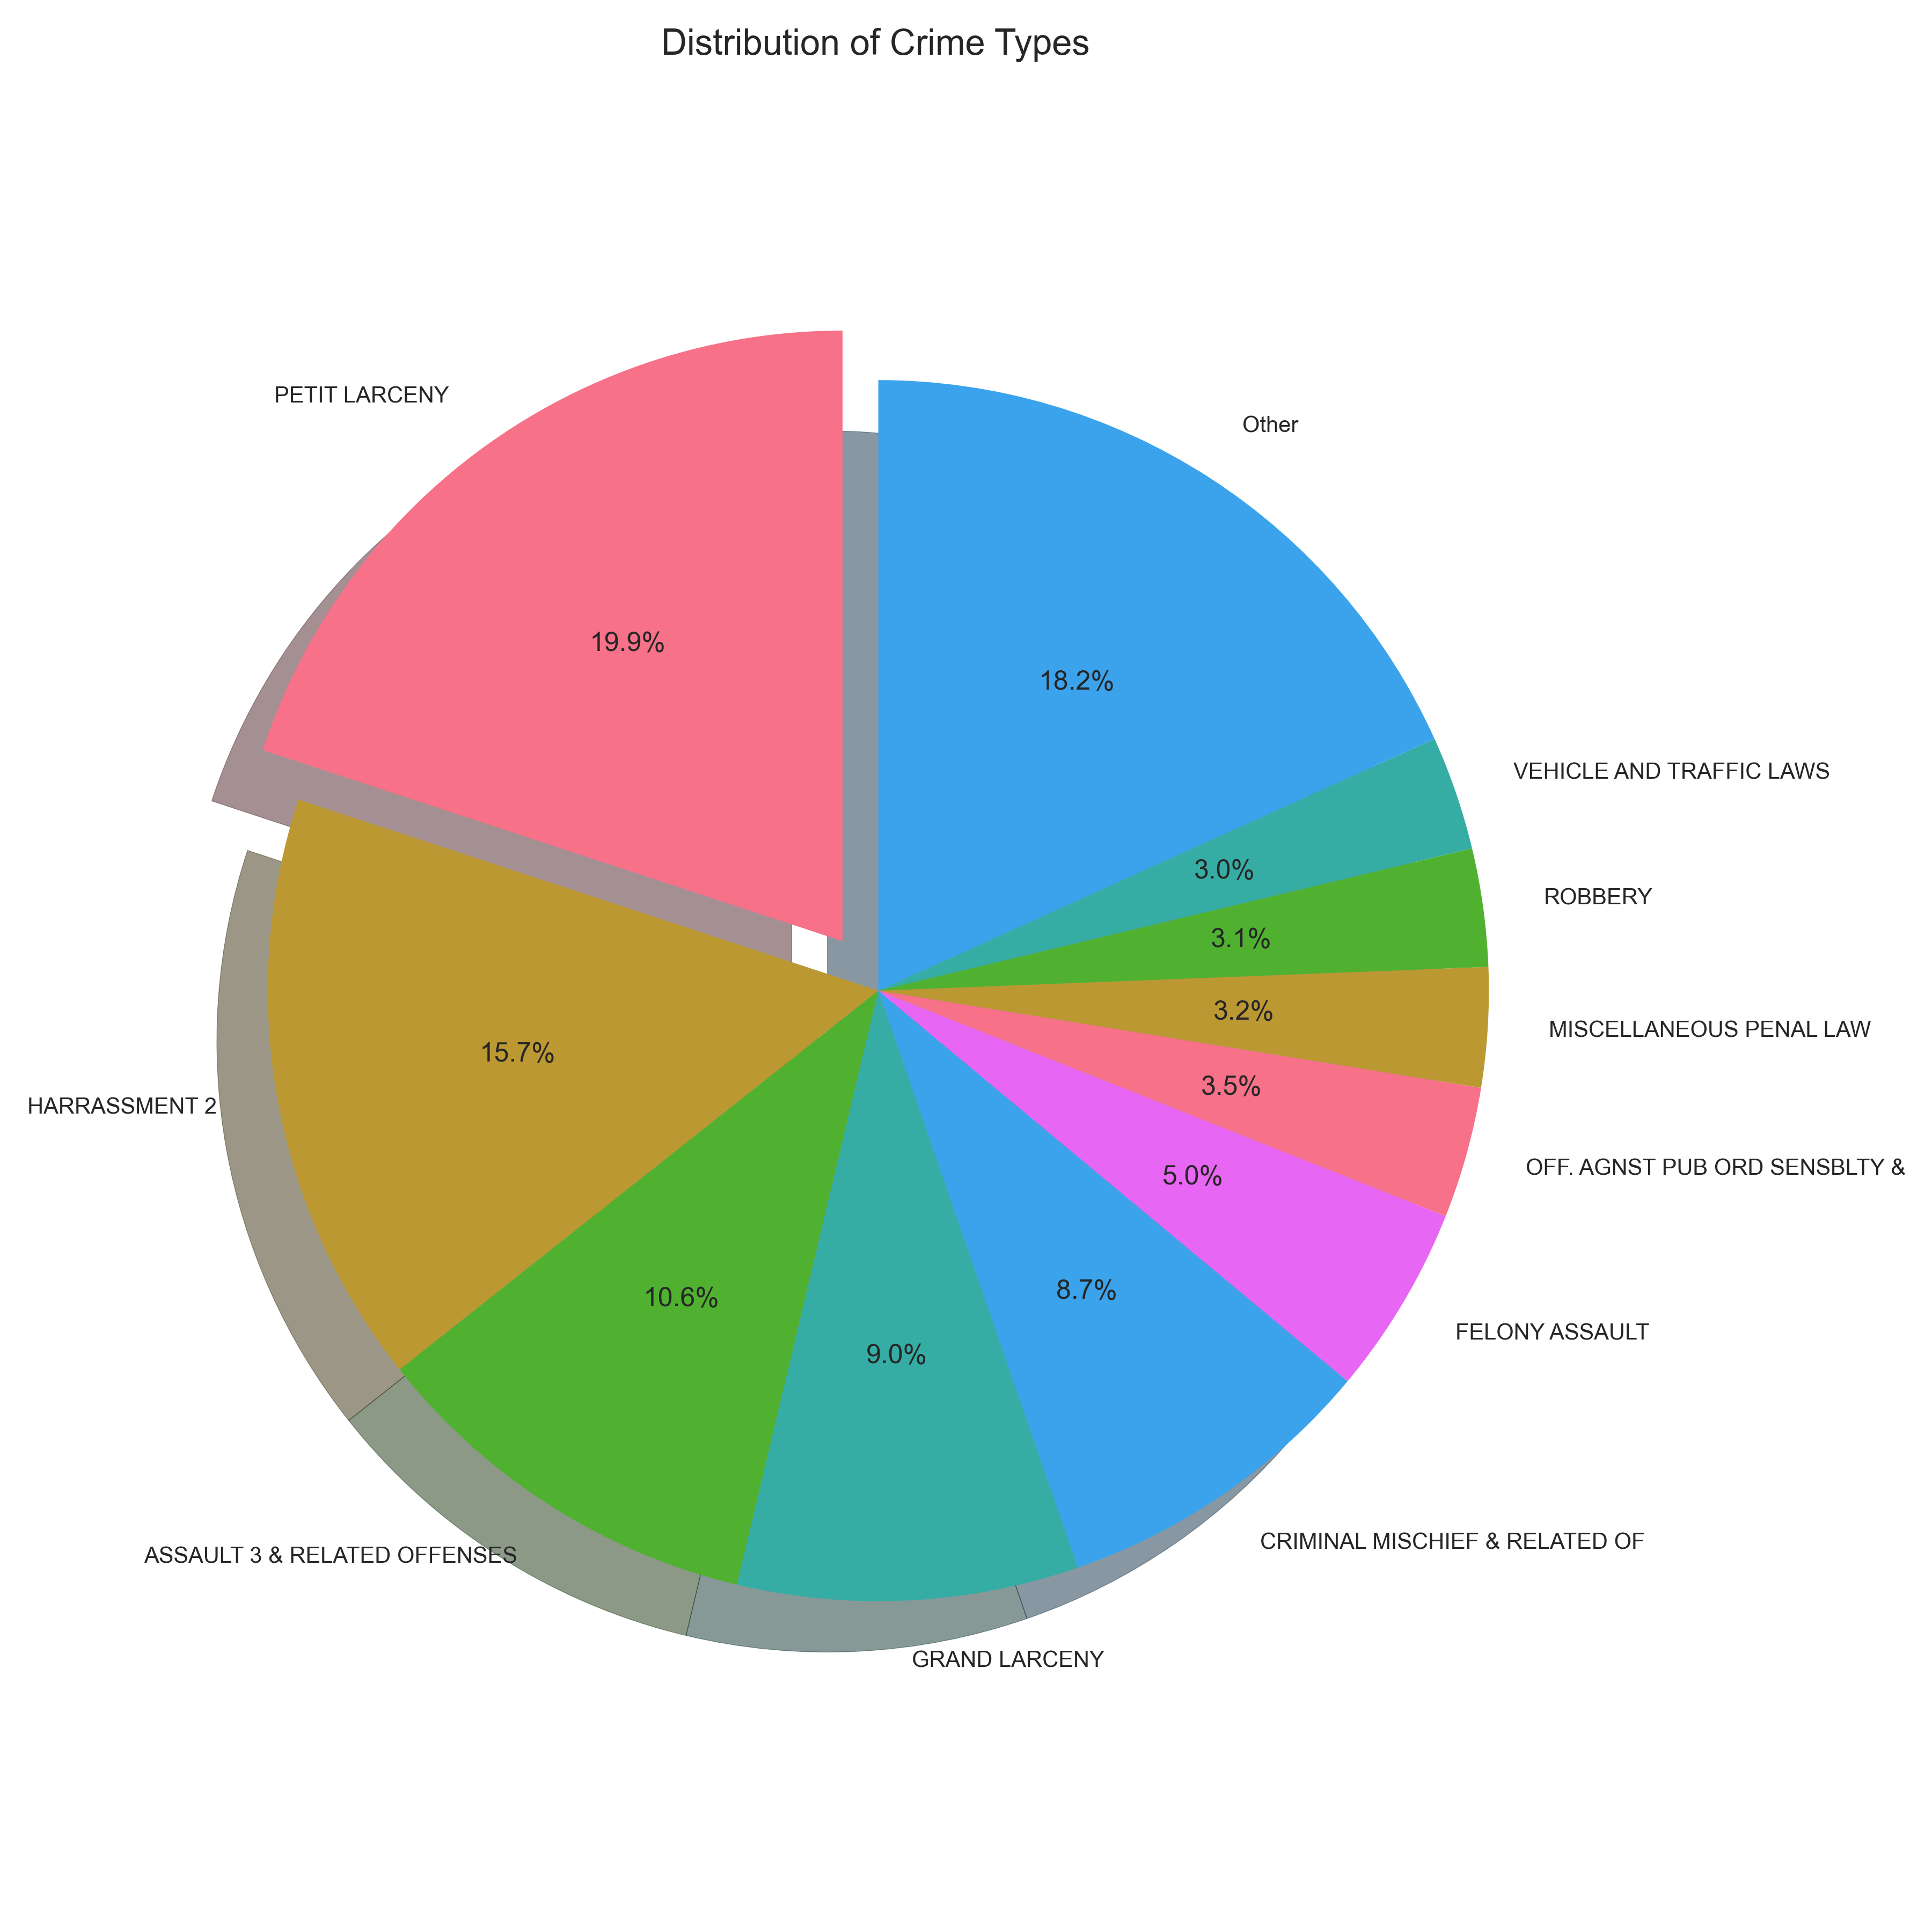
\includegraphics[width=0.45\textwidth]{crime_types_pie_chart.png}
\caption{Crime types distribution.}
\end{figure}

\section{Appendix B: Reproducibility and Artifacts}
Key artifacts available in the repository for verification and integration:
\begin{itemize}
	\item Final production model: \texttt{JupyterOutputs/Classification (Final)/LogisticRegression\_production\_model.joblib}
	\item Final preprocessing pipeline(s): \texttt{JupyterOutputs/Classification (Preprocessing)/*.joblib}
	\item Full evaluation JSON: \texttt{JupyterOutputs/Classification (Final)/LogisticRegression\_evaluation\_report.json}
	\item Threshold tuning: \texttt{JupyterOutputs/Classification (Tuning)/LogisticRegression\_threshold\_optimization.json} and PNG
	\item Best hyperparameters: \texttt{JupyterOutputs/Classification (Tuning)/LogisticRegression\_best\_params.json}
	\item Final dataset metadata: \texttt{JupyterOutputs/Final/final\_dataset\_metadata.json}
\end{itemize}

Environment details, seeds, and full API specifications: \texttt{<INFO TO ADD>}.
Future developments could include:
\begin{itemize}
\item City-wide deployment for comprehensive safety monitoring.
\item Integration with smart city infrastructure.
\item Personalized risk profiles based on user behavior.
\item Collaboration with tourism industry for enhanced visitor experiences.
\end{itemize}

\end{document}